\documentclass[12pt, openany]{book}
\usepackage[italian]{babel}
\usepackage{xcolor}
\usepackage{float}
\usepackage{graphicx}
\usepackage{listings}
\usepackage{caption}
\newcommand\myworries[1]{\textcolor{red}{#1}}

\definecolor{codegreen}{rgb}{0,0.6,0}
\definecolor{codegray}{rgb}{0.5,0.5,0.5}
\definecolor{codepurple}{rgb}{0.58,0,0.82}
\definecolor{backcolour}{rgb}{0.95,0.95,0.92}
\renewcommand{\lstlistingname}{Script}
\lstdefinestyle{mystyle}{
	backgroundcolor=\color{backcolour},   
	commentstyle=\color{codegreen},
	keywordstyle=\color{magenta},
	numberstyle=\tiny\color{codegray},
	stringstyle=\color{codepurple},
	basicstyle=\ttfamily\footnotesize,
	breakatwhitespace=false,         
	breaklines=true,                 
	captionpos=b,                    
	keepspaces=true,                 
	numbers=left,                    
	numbersep=5pt,                  
	showspaces=false,                
	showstringspaces=false,
	showtabs=false,                  
	tabsize=2
}

\lstset{style=mystyle}

\begin{document}
	\chapter*{Introduzione}	
		Il CoronaVirus-19, abbreviato \textsc{CoViD-19}, è un virus trovato per la prima volta nella città di Wuhan, in Cina. Esso è conosciuto anche come \emph{Malattia respiratoria acuta}, abbreviato in \textsc{SARS-CoV-2}, dato che è un virus che come principale metodo di trasmissione utilizza le vie aeree, ha avuto vita facile nel diffondersi velocemente, in effetti tutti respiriamo. In breve tempo si è passati dall'isolamento della Cina al doverlo definire \textbf{pandemia} e quindi passare ad un isolamento globale.
		Per la sua facilità di diffusione e per la sua pericolosità per alcuni soggetti più deboli, è stato necessario modificare lo stile di vita a cui si era abituati, iniziando con i lockdown, dovendo passare alla didattica a distanza, abbiamo visto l'economia rallentare, nei casi peggiori crollare. Abbiamo perso la quasi totalità del contatto umano per via  della chiusura temporanea di aziende e luoghi definiti "non di prima necessità".
		Questa situazione ha dato una motivazione per effettuare studi e ricerche in questo ambito, sia per ridurre i sintomi del virus, in buona parte già sta avvenendo con i vari vaccini, sia per permettere alle persone di incontrarsi e lavorare come prima della pandemia trovando metodi per ridurre i contagi come le mascherine. In Italia stiamo allentando la presa sulle restrizioni grazie anche all'avvento del \textsc{GreenPass} il quale permette di certificare che si è vaccinati o che si hanno gli anticorpi dovuti ad un'infezione da \textsc{CoViD-19}. Questo però non ferma il contagio dato che il vaccino permette agli individui di avere sintomi più lievi, ma è comunque possibile essere contagiati e diffondere il virus. 
		Uno degli aspetti che coinvolge un po' tutte le persone, sia per divertimento che per lavoro è il trasporto pubblico. Non tutti hanno un mezzo di trasporto proprio o per molti addirittura non conviene, basti pensare alle grandi città con lunghe code per il traffico a tal punto da fare prima a far il tragitto a piedi. Quindi molti optano per i trasporti pubblici ma qui è dove avvengono i principali contagi dovuti ai luoghi chiusi, stretti e poco arieggiati che impediscono di seguire perfettamente le normative dettate dal governo e dall'Organizzazione Mondiale della Sanità (OMS); questo è uno dei principali motivi del lavoro di tesi.\\
		L'obbiettivo del progetto di tesi è quello di creare una simulazione ad agenti estendibile a diversi tipi di percorsi e abitudini cittadine diverse, da cui recuperare dati sulle persone e sui contagi che avvengono su un mezzo di trasporto pubblico (nel nostro caso si tratta di un autobus). La simulazione è stata realizzata interamente in \textsc{Unity3D},un motore grafico di che consente lo sviluppo di contenuti interattivi digitali, sia 2D che 3D, come ad esempio videogiochi e simulazioni. Sono stati anche utilizzati tool ed algoritmi per risolvere  vari problemi, come ad esempio abbiamo utilizzato \textsc{A* Pathfinding Project} a cura di Aron Granberg per il calcolo del percorso degli agenti. 
		\\Gli agenti vengono distinti in:
		\begin{itemize}
			\item Sano, indicato in verde
			\item Contagioso, indicato in rosso
			\item Infetto, indicato in giallo
			
		\end{itemize} 
		Come è visibile nella Figura \ref{fig:agenti}
	\begin{figure}[H]
		\centering
		\includegraphics[width=1\linewidth]{"Immagini/Agenti"}
		\caption{Stati degli agenti}
		\label{fig:agenti}
	\end{figure}		
		I dati sul numero di pendolari della tratta sono stati presi da un articolo riguardante uno studio pre-pandemia sui viaggiatori della cittadina giapponese di Obuse \cite{Obuse}, della quale è stato preso il percorso della tratta del bus. La simulazione permette di selezionare la percentuale di contagiati iniziale e la percentuale di infezione del virus in modo tale da effettuare facilmente diversi test. Il numero di persone alle fermate è selezionabile per ogni singola fermata in modo tale da poter essere utilizzate in diversi percorsi o più semplicemente applicarlo alle stime dei pendolari attuali.\\
		All'avvio della simulazione viene generato un file .csv che verrà riempito per ogni tratta del bus con le informazioni generate sugli agenti, come il numero i agenti totali, quelli contagiosi, quelli infetti e quelli sani.
		\\
		La tesi sarà suddivisa nelle seguenti sezioni:
		\begin{itemize}
			\item \textbf{Stato dell'arte}: verrà mostrato lo stato delle ricerche sulla diffusione del \textsc{CoViD-19} in ambito di trasporti pubblici, citando elaborati e mostrandone i punti di forza e le limitatezze.
			\item \textbf{Presentazione delle tecnologie}: in questa sezione verrà mostrato in dettaglio le tecnologie utilizzate per la creazione della simulazione.
			\item\textbf{Simulazione nel dettaglio}: verrà mostrato il lavoro svolto per la realizzazione della simulazione mostrando in dettaglio i vari oggetti, come sono stati utilizzati i tool e il lavoro svolto senza tool.
			\item\textbf{Risultati ottenuti}: verrà mostrato i risultati ottenuti da vari test della simulazione.
			\item\textbf{Conclusione e sviluppi futuri}: si analizzeranno le limitazioni del lavoro allo stato attuale e si metteranno in risalto idee per sviluppi futuri
		\end{itemize}
	\chapter{Stato dell'arte}
		Dalla scoperta del salto di specie effettuato dal \textsc{CoViD-19} sull'essere umano ad oggi ci sono stati innumerevoli studi, ricerche su vari aspetti della malattia, sul suo impatto sulla società in ambito politico, sociale ed economico. Ci sono anche varie simulazioni sulla sua diffusione in varie situazioni come trasporti pubblici, uffici, ospedali, locali pubblici. \\
		Come primo articolo si parlerà di \emph{"Simulaion-based Estimation of the Spread of COVID-19 in Iran"} \cite{Iran} pubblicato il 27 Marzo 2020 su medRxiv. Come primo luogo l'articolo mette in luce i problemi dovuti ai dati provenienti dai vari paesi colpiti dal virus, definendoli altamente inaffidabili perché non tengono conto che i sintomi lievi del \textsc{CoViD-19} sono assimilabili al raffreddore stagionale o alla comune influenza, in più molti testi vengono effettuati tramite screening limitati, un metodo per effettuare esami a tappeto allo scopo di individuare una malattia. Tutti questi dati non vengono combinati con le statistiche ufficiali sulla diffusione del virus e si va quindi a sottovalutare la quantità di infetti.
		Lo studio è stato effettuato sulla diffusione del virus in Iran nei primi mesi del 2020.\\
		È stato sviluppato un modello dinamico per fornire un quadro affidabile dello stato della malattia basandosi sui dati esistenti. Il modello si basa sul framework \textbf{SEIR}(Suscettibile, Esposto, Infetto, Ricoverato); 
		\begin{figure}[H]
			\centering
			\includegraphics[width=1\linewidth]{"Immagini/SEIR"}
			\caption{Questo è la rappresentazione di un modello SEIR }
			\label{fig:SEIR}
		\end{figure}
		I modelli matematici, in epidemiologia, sono modelli simbolici costituiti da una o più equazioni che considerano diversi parametri per prevedere l'andamento di una malattia in diverse condizioni ambientali o per calcolare il rischio di morte o l'aspettativa di vita nel corso di una pandemia di specifiche entità. SEIR è uno di questi modelli matematici, esso considera il periodo di incubazione durante il quale un individuo è infetto ma non contagioso, in questo caso si trova nello stato di \emph{"Esposto"}, questo è il principale motivo per cui è stato scelto questo modello, tenendo conto il periodo di incubazione del \textsc{CoViD-19} che ha un massimo di 14 giorni.\\
		Come primo parametro è stato registrata la frequenza di contatti medi tra persone man mano che venivano segnalati i decessi, poi sono stati differenziati i casi segnalati dai casi effettivi e di come questa differenza cambia con l'andare dell'epidemia(all'epoca ancora definibile epidemia). Nel modello sono stati utilizzati sia dati ufficiali che dati stimati dalla comunità medica in modo tale da ricostruire un quadro più completo della situazione epidemica. Questi dati vengono raccolti per poi passare ad un simulazione con metodo \emph{Monte Carlo}; è una classe di metodi computazionali basati sul campionamento casuale per ottenere risultati numerici, questo metodo è utilizzato per trarre stime attraverso simulazioni.
		Da quest'analisi sono state trovate sei possibili situazioni della diffusione della malattia in relazione ad effetti stagionali e misure di distanziamento sociale.\\
		I risultati dello studio mostra che il vero numero di casi probabilmente è molto più grande di quello effettivamente registrato, quasi il doppio degli infetti. Lo studio avverte sul fatto che i dati potrebbero dichiarare molti meno casi di quelli che sono nella realtà portando la popolazione e i governi a sottovalutare la situazione.
		\\
		\\
		Il prossimo documento di cui si parlerà è  \emph{"How simulation modelling can help reduce the impact of COVID-19"} \cite{Simulazioni} a cura della professoressa Christine Currie pubblicato dal \textsc{CORMSIS}, centro di ricerca operativa e statistica dell'Università del \emph{Southamoton}, il 15 Aprile 2020 su Taylor\&Francis Online il quale tratta dei vari modelli utilizzati dai governi e dall'Organizzazione Mondiale della Sanità per decidere le migliori strategie per debellare la minaccia del \textsc{CoViD-19}. I modelli utilizzati sono modelli epidemiologici volti a comprendere la diffusione della malattia. In quest'articolo verranno discussi di come i vari modelli di simulazione potrebbe aiutare a prendere decisioni.
		Il presente articolo presenta due obbiettivi, il primo è dare una guida ai diversi modelli di simulazioni e quali tipi possono essere utili a prendere decisioni durante un'emergenza sanitaria; il secondo è una \emph{"Chiamata alle armi"} dei modellatori di simulazioni per migliorare le ricerche.
		I modelli di tipo epidemiologico sono un'idea per predire il numero di nuovi casi identificando le migliori misure per ridurre i contagi, ma non aiutano ad organizzare l'organizzazione delle terapie intensive all'interno degli ospedali. Come nel paper precedente anche nel presente si indica il modello \emph{SEIR} come il modello più popolare per descrivere l'attuale pandemia per via del tempo di incubazione dato dallo stato di "Exposed".\\
		Questo paper considera quattro metodi di modellazione:
		\begin{itemize}
			\item \emph{Sistemi dinamici}: è un modello basato su equazioni differenziali che rappresentano azioni nel mondo.
			\item \emph{Modello basato ad agenti} può essere utilizzato per modellare l'interazione tra gli individui. In questi modelli utilizzati per monitorare la diffusione di una malattia è molto importante gestire le reti sociali e i movimenti nello spazio.
			\item \emph{Simulazione ad eventi discreti}, il sistema è rappresentato, nella sua evoluzione nel tempo, con variabili che cambiano istantaneamente il loro valore in ben definiti istanti di tempo appartenenti ad un insieme numerabili, questi istanti sono definiti eventi.
			\item \emph{Simulazione ibrida}: sono modelli che combinano due o più tecniche di modellazione citate precedentemente.
		\end{itemize}
	Dato che le simulazioni sviluppate con i metodi descritti in precedenza possono diventare molto complesse e richiedere tempo per l'esecuzione sono state sviluppate le simulazioni distribuite, le quali permettono di collegare più simulazioni in una singola in scala maggiore permettendo una velocità maggiore.\\ 
	Di seguito il presente paper introduce le tipologie di decisioni che sono state prese grazie all'utilizzo di simulazioni durante la pandemia da CoViD-19; esse vengono divise in tre sezioni:
	\begin{itemize}
		\item \emph{Decisioni che hanno avuto effetto sulla diffusione del virus.}
		\item \emph{Decisioni che riguardano la gestione delle risorse.}
		\item \emph{Decisioni sulla salute della popolazione.}
	\end{itemize}
	\begin{figure}[H]
		\centering
		\includegraphics[width=0.8\linewidth]{"Immagini/Decisioni"}
		\caption{Questo è uno schema sulle decisioni consigliate dal risultato di diverse tipologie di modelli per le simulazioni.}
		\label{fig:decisioni}
	\end{figure}
 	La Figura \ref{fig:decisioni} mette in luce le diverse decisioni suggerite dalle quattro tipologie di modelli in base a scala organizzativa e fase di emergenza.
	Ora andiamo più nel dettaglio nelle decisioni per evitare la diffusione del virus descritte nel presente paper.\\
	Come prima decisione possibile abbiamo quella della \emph{quarantena}, questo per evitare del tutto la diffusione del virus. Questa decisione è d'obbligo una volta individuato un caso di corona virus, questo fino alla sua completa guarigione in modo tale da non poter contagiare nessuno. L'articolo cita un articolo del 2016 intitolato \emph{"The Ebola crisis and the corresponding public behavior: A system dynamics approach"} il quale dimostra di come la messa in quarantena dei casi di \textsc{ebola} ha avuto un impatto importante su combattere la malattia; questo però non è applicabile così facilmente alla pandemia da corona virus dato che i sintomi dell'\textsc{ebola} sono ben visibili sulla pelle dei malcapitati, a differenza di quelli da \textsc{CoViD-19} che possono anche essere lievi o assenti.\\
	Una seconda decisione che ha avuto un grande impatto sul nostro stile di vita, ma allo stesso è stato di grande aiuto per combattere la diffusione del virus sono le misure di \emph{distanziamento sociale}. Per distanziamento sociale si intendono quei comportamenti nel quale riduciamo, in parte, il contatto umano in modo tale da essere sicuri di essere contagiati o di contagiare e quindi puntare a ridurre la crescita della curva dei contagi. Esempi di distanziamento sociale possono essere: \begin{itemize}
		\item mantenere una distanza di sicurezza di circa due metri in modo tale da non far arrivare gocce di saliva alla persona con cui stiamo colloquiando
		\item lavorare da casa quando è possibile, infatti molte aziende sono passate allo smart-working, in modo tale da continuare a lavorare tranquillamente anche da casa.
		\item Cancellare eventi i quali prevedono un elevato numero di persone.
		\item chiudere le scuole e optare per le lezioni in remoto.
		\item evitare di incontrare fisicamente amici e parenti.
	\end{itemize}
	Una decisione molto più drastica delle due precedenti è il lock-down imposto dal governo in modo tale da costringere la popolazione al distanziamento sociale e a lasciare le abitazioni sono in caso di prima necessità, come andare a fare la spesa, andare a lavorare ed uscire per motivi di salute. Per ovviare a problemi legati all'economia ogni governo può includere una soglia di valori sul quando rilassare le restrizioni in modo tale da permettere ai lavoratori che non eseguono un lavoro considerato di \emph{"Prima necessità"} di lavorare facendo girare l'economia.\\
	In conclusione il documento lascia un appello definendolo \emph{"The call to arms"} invitando a sviluppare simulazioni in merito alla diffusione e ai comportamenti per combattere la diffusione del virus in modo tale da supportare la ricerca, per poi fare l'esempio dei \emph{"codebreakers"} britannici insieme ad \emph{Alan Turing}, durante la Seconda Guerra Mondiale, decriptarono Enigma mostrando che l'unione di un buon team risolve problemi difficili.\\
	Lo sviluppo delle simulazioni si è dimostrato essere molto efficace, basti pensare al fatto che questo paper è stato redatto il 27 Marzo 2020 e seguendo le decisioni suggerite dalle simulazioni stiamo pian piano tornando alla normalità.\\
	
	Esistono numerosi studi che utilizzano simulazioni riguardo al \textsc{CoViD-19} per varie motivazioni, quali: allo scopo di fornire un modello per comprendere al meglio le dinamiche spazio-temporali della diffusione della pandemia \cite{Singapore}; oppure allo scopo di predire i rischi nel rimuovere le limitazioni di movimento alla popolazione illustrando anche l'efficacia delle mascherine in ambienti di simulazioni a lungo termine \cite{Madrid}; o ancora studi con dati meno accurati ottenuti con sondaggi telefonici durante le prime fasi di pandemia per avere dati aggiuntivi rispetto a quelli forniti da istituzioni governative \cite{HongKong}.
	\chapter{Presentazione delle tecnologie}
	In questo capitolo verranno mostrate, nel dettaglio, tutte le tecnologie utilizzate per la realizzazione della simulazione.
	\section{Unity}
	In primo luogo abbiamo la base della simulazione, \textsc{Unity} \cite{Unity}, un motore grafico multipiattaforma sviluppato da \emph{Unity Technologies} utilizzato per lo sviluppo di contenuti interattivi, quali: videogiochi; simulazioni; esperienze interattive con dispositivi di realtà aumentata. \\
	Possiamo dividere \textsc{Unity} in due sottosistemi,\emph{ Unity Editor} e \emph{Unity Engine}. 
	\subsection{Unity Editor}
	Con \emph{Unity Editor} si intende l'interfaccia grafica di \textsc{Unity}, la quale è costruita per rendere facili le interazioni da parte dell'utente, essa è completamente modificabile a piacere dell'utente che la possibilità di salvare il suo editor in profili per ogni situazione.\\
	Ora parleremo delle diverse componenti della UI dell'editor di \textsc{Unity}.
	\subsubsection{Inspector}
	Ogni oggetto in \textsc{Unity} è descritto dal concetto di \textsc{GameObject}, il quale identifica ogni oggetto in \textsc{Unity}. Ogni \textsc{GameObject} è decorato dai cosidetti \emph{Components}, i quali possono essere di diverso genere e comprendono \emph{mesh}, script(in C\#), animazioni, \textsc{rigidBody}(il quale gestisce le componenti fisiche di un \textsc{GameObject}) e molti altri.
	\begin{figure}[H]
		\centering
		\includegraphics[width=1\linewidth]{"Immagini/Inspector"}
		\caption{Questo è l'inspector di un semplice cubo in Unity}
		\label{fig:Inspector}
	\end{figure}

	Come è possibile vedere nella figura \ref{fig:Inspector} l'inspector permette di aggiungere, rimuovere e modificare i \emph{component} dei \textsc{GameObject}.
	\subsubsection{Hierarchy}
	L'Hierarchy contiene tutti gli oggetti di scena, come si può intuire dal nome, gli oggetti vengono mostrati tramite una gerarchia ad albero dove come radice abbiamo la \emph{scena}.
	\begin{figure}[H]
		\centering
		\includegraphics[width=1\linewidth]{"Immagini/Hierarchy"}
		\caption{Questa è l'Hierarchy della simulazione.}
		\label{fig:Hierarchy}
	\end{figure}
	Come si può vedere dalla figura \ref{fig:Hierarchy} possiamo vedere come radice abbiamo l'oggetto "Obuse" che è la scena principale della simulazione e come figli ci sono tutti gli oggetti di scena.
	\subsubsection{Project}
	La finestra \emph{Project} permette di gestire la directory del progetto nella quale sono presenti script, prefab, modelli, texture, file audio e scene.
	\begin{figure}[H]
		\centering
		\includegraphics[width=1\linewidth]{"Immagini/Project"}
		\caption{Questa è la finestra Project della simulazione}
		\label{fig:Project}	
	\end{figure}
	Come è possibile vedere nella figura \ref{fig:Project} il progetto è diviso in diverse cartelle per avere un'organizzazione migliore delle risorse.
	
	\subsubsection{Scene}
		La finestra \emph{"Scene"} rappresenta la scena corrente, tutti i \textsc{GameObject} che sono nell'Hierarchy, come detto precedentemente, sono nella scena corrente. Dalla scena è possibile manipolare i \textsc{GameObject} con strumenti di traslazione, rotazione e ridimensionamento. Tramite il mouse e la tastiera possiamo navigare con facilità nella scena oppure per essere più rapidi è possibile fare focus sull'oggetto selezionato, o dall'Hierarchy o dalla scena, premendo il tasto \emph{F}.
		\begin{figure}[H]
			\centering
			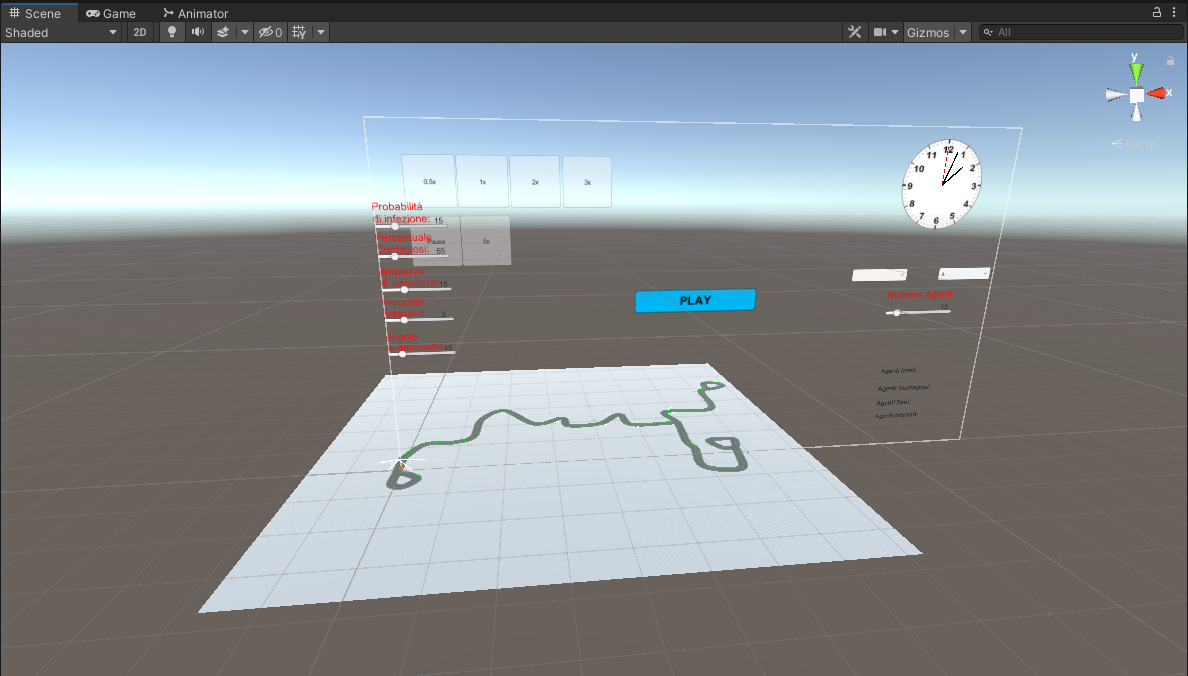
\includegraphics[width=0.72\linewidth]{"Immagini/Scene.png"}
			\caption{Questa è la scena della simulazione}
			\label{fig:Scene}
		\end{figure}
	Dalla figura \ref{fig:Scene} possiamo vedere tutta la scena della simulazione, compresa di gui (Delineata dal quadrato con bordi bianchi)
	\subsubsection{Game}
		La finestra \emph{Game} viene utilizzata quando si esegue il progetto, si passa alla finestra di game con la quale è possibile effettuare testi direttamente da \textsc{Unity}. Allo stesso tempo è possibile modificare parametri dalla scena e dall'Inspector mentre il \textsc{Game} è in esecuzione.
		\begin{figure}[H]
			\centering
			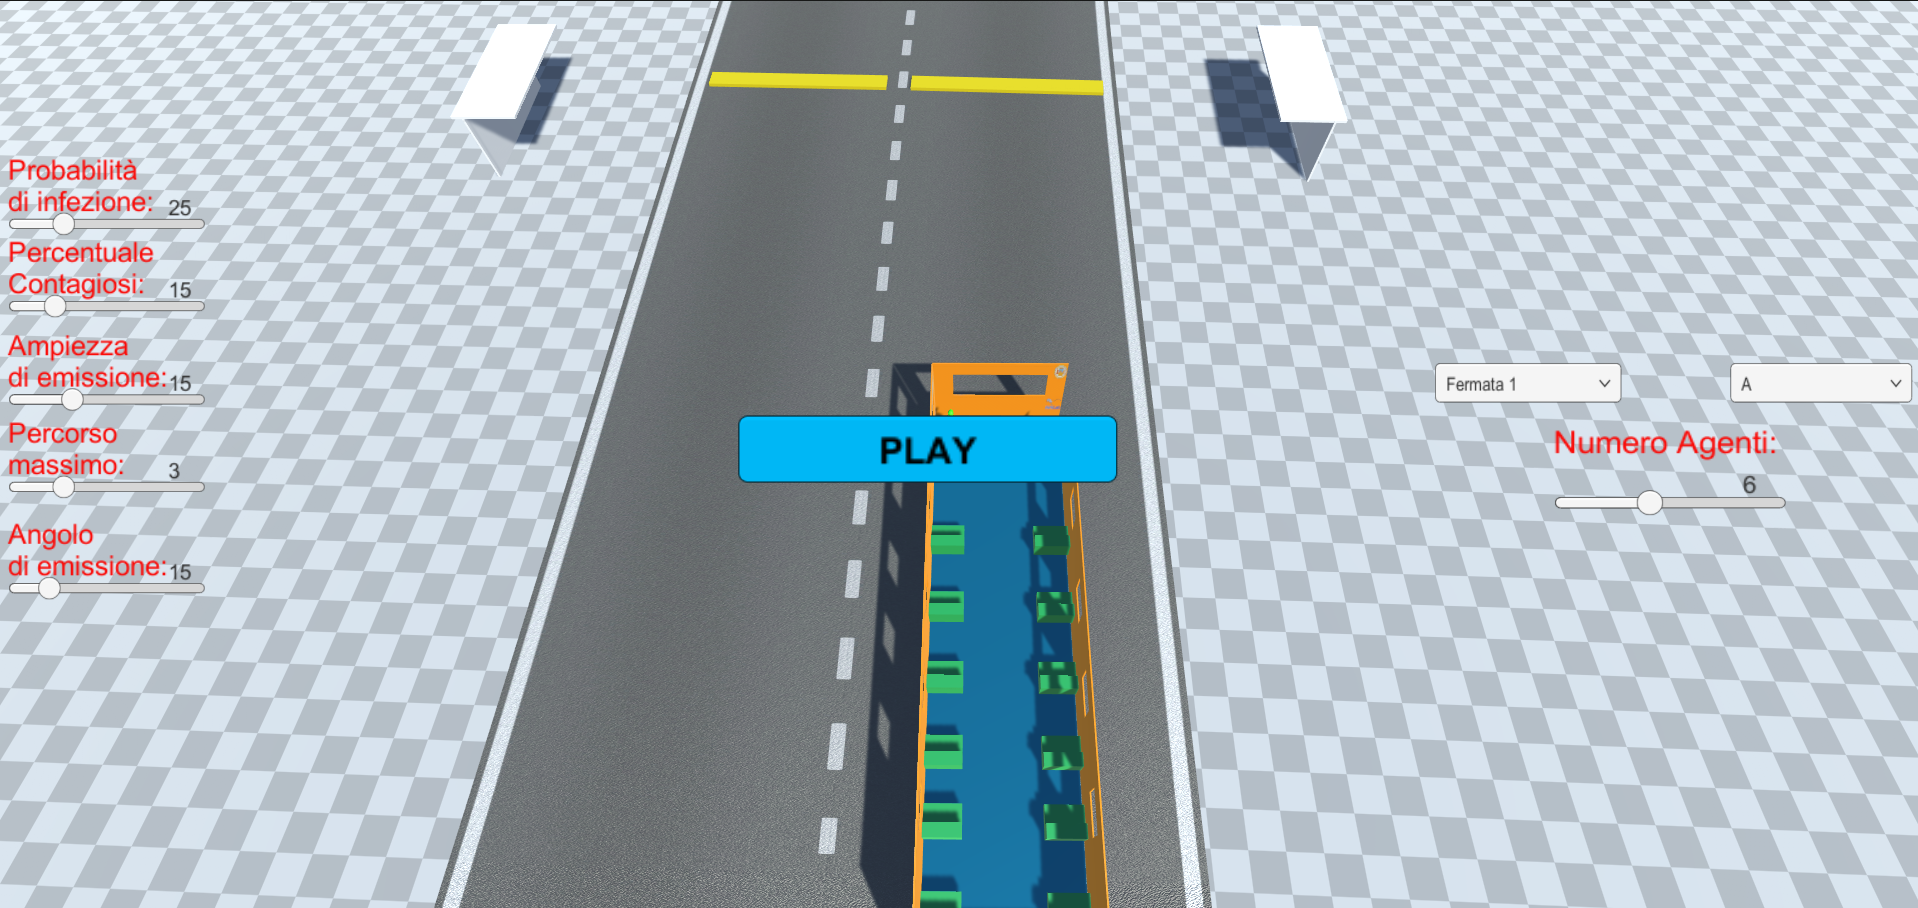
\includegraphics[width=1\linewidth]{"Immagini/PausedGame.png"}
			\caption{Questo è il game in pausa}
			\label{fig:PausedGame}
		\end{figure}
	Nella figura \ref{fig:PausedGame} viene mostrato il game quando è in pausa prima di iniziare, a sinistra si possono vedere vari slider per la gestione dei parametri della simulazione, mentre a destra abbiamo dei menù a tendina per la selezione degli agenti nelle varie fermate.
	\begin{figure}[H]
		\centering
		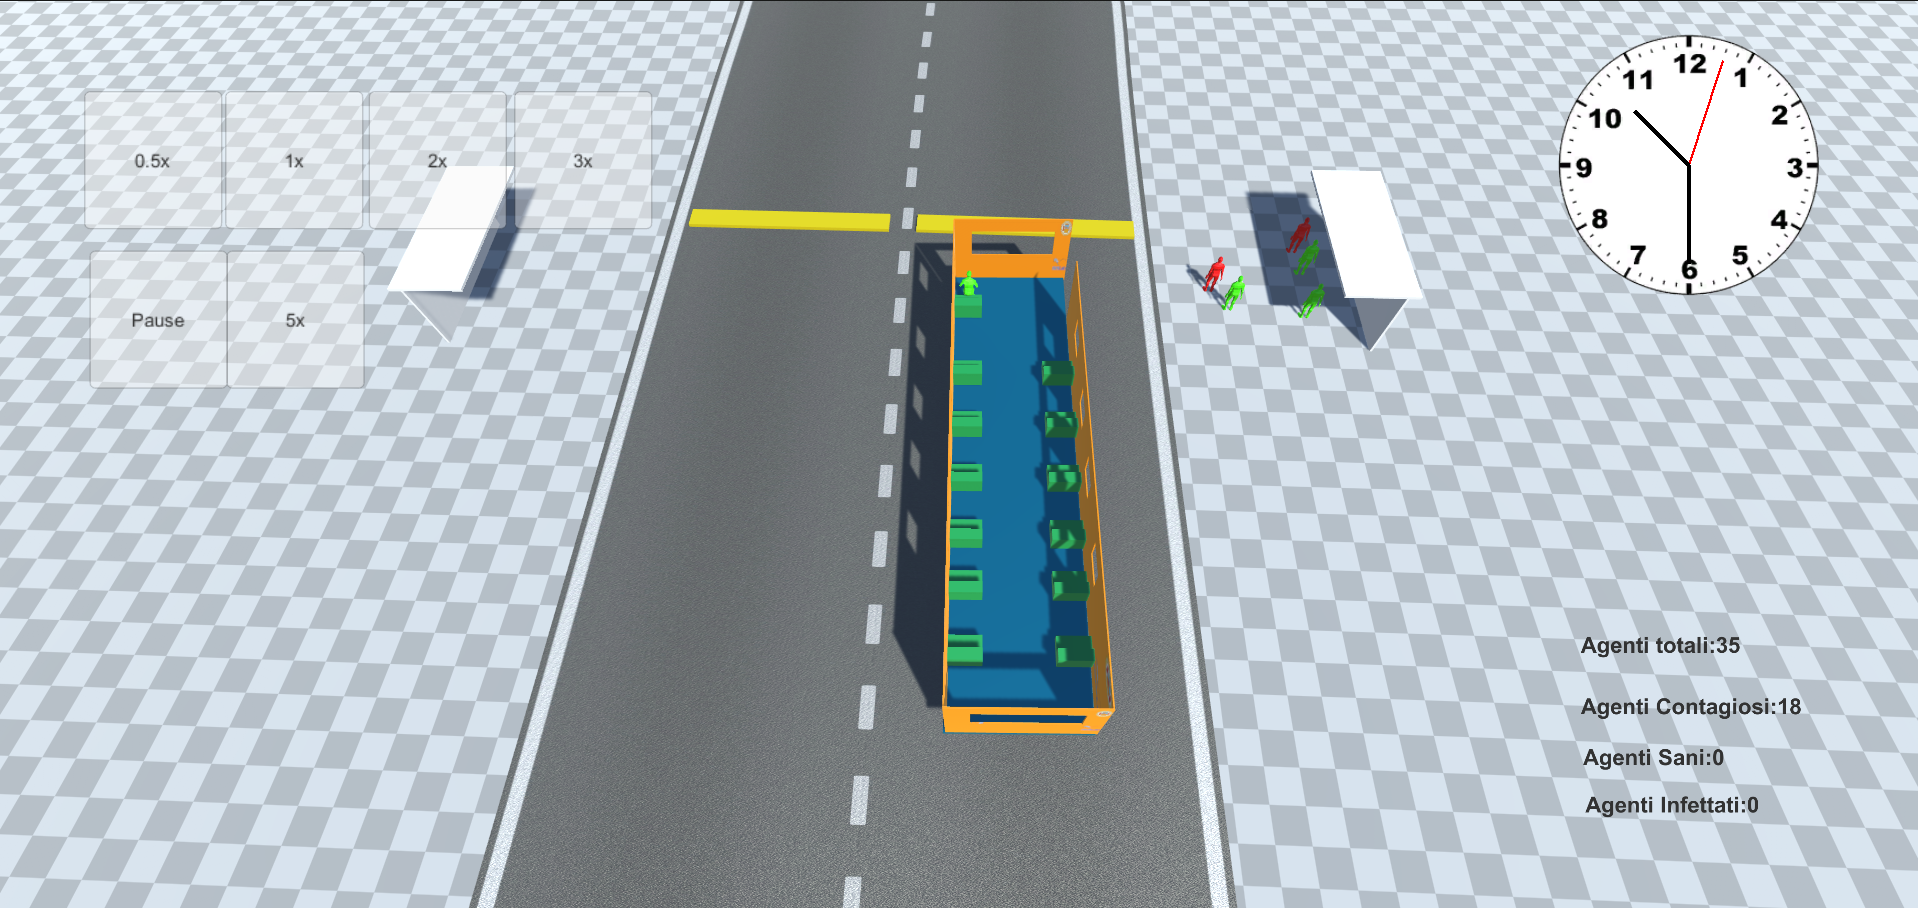
\includegraphics[width=1\linewidth]{"Immagini/PlayingGame.png"}
		\caption{Questo è il game una volta iniziato}
		\label{fig:PlayingGame}
	\end{figure}
	Nella figura \ref{fig:PlayingGame} viene mostrato il game in play, quindi cambia l'interfaccia, a sinistra abbiamo i vari bottoni per la gestione della velocità della simulazione, in alto a destra abbiamo l'orologio che scandisce il tempo della simulazione; il quale rispetta il tempo reale della tratta di Obuse e infine, in basso a destra, abbiamo i dati sugli agenti.
	\subsubsection{Animation e Animator}
		Come è stato detto in precedenza, gli agenti della simulazione sono completamente animati, quindi ora parleremo di Animazioni e \textsc{Animator}. La finestra \textsc{Animator} permette di creare e modificare le animazioni tramite la timeline dell'oggetto da animare. 
		\begin{figure}[H]
			\centering
			\includegraphics[width=0.8\linewidth]{"Immagini/Animation"}
			\caption{Questa è la finestra Animation dell'animazione \emph{"Sit to Stand"} dell'agente che gli permette di sedersi sull'autobus.}
			\label{fig:Animation}
		\end{figure}
		Come è possibile vedere dalla figura \ref{fig:Animation} sulla sinistra abbiamo le sezioni dell'agente da animare, in alto abbiamo la timeline e al centro abbiamo i frame corrispondenti alle sezioni in corrispondenza del frame nella timeline.\\
		Tutte le animazioni sono gestite dal component \textsc{Animator}, una macchina a stati finiti in grado di gestire differenti stati e passare da uno stato all'altro attraverso transizioni. 
		\begin{figure}[H]
			\centering
			\includegraphics[width=0.8\linewidth]{"Immagini/Animator"}
			\caption{Questo è il component animator.}
			\label{fig:Animator}
		\end{figure}
		Dalla figura \ref{fig:Animator} è possibile vedere, sulla sinistra, la macchina a stati finiti che è l'\textsc{animator}; sulla destra invece abbiamo il focus di una transizione, più precisamente dallo stato  \emph{Dark Dance 3} a \emph{Dark Dance 4} la quale avviene quando la variabile \emph{mode} ha valore pari a 13, come è possibile vedere nella sezione \emph{conditions}.
	\subsection{Unity Engine}
	Abbiamo parlato della parte di interfaccia utente di \textsc{Unity}, ora parleremo di quello che c'è dietro la realizzazione di un applicativo in \textsc{Unity}.
	Il motore di \textsc{Unity} permette di gestire la fisica del mondo virtuale in modo semplice aggiungendo vari \textsc{component} ai \textsc{GameObject}, come il \textsc{Rigidbody} o i \textsc{Collider}. Più nello specifico il \textsc{Rigidbody} è un componente che permette ai \textsc{GameObject} di agire in risposta alle forze del mondo di gioco; ad esempio è possibile indicare se un oggetto deve essere soggetto alla gravità oppure è possibile bloccare rotazione o traslazione su uno specifico asse, tutto questo è possibile selezionarle all'interno dell'Inspector o tramite scripting in \textsc{C\#}.\\
	I \textsc{Collider}, invece, permettono di gestire la collisione tra gli oggetti, più nello specifico permette di ascoltare le collisioni che avvengono tra \textsc{Collider} e \textsc{Rigidbody}. I \textsc{Collider} hanno diverse forme per addatarli ad ogni situazione; ad esempio abbiamo il \textsc{BoxCollider}, \textsc{SphereCollider}, \textsc{MeshCollider}, \textsc{CapsuleCollider}.
	\begin{figure}[H]
		\centering
		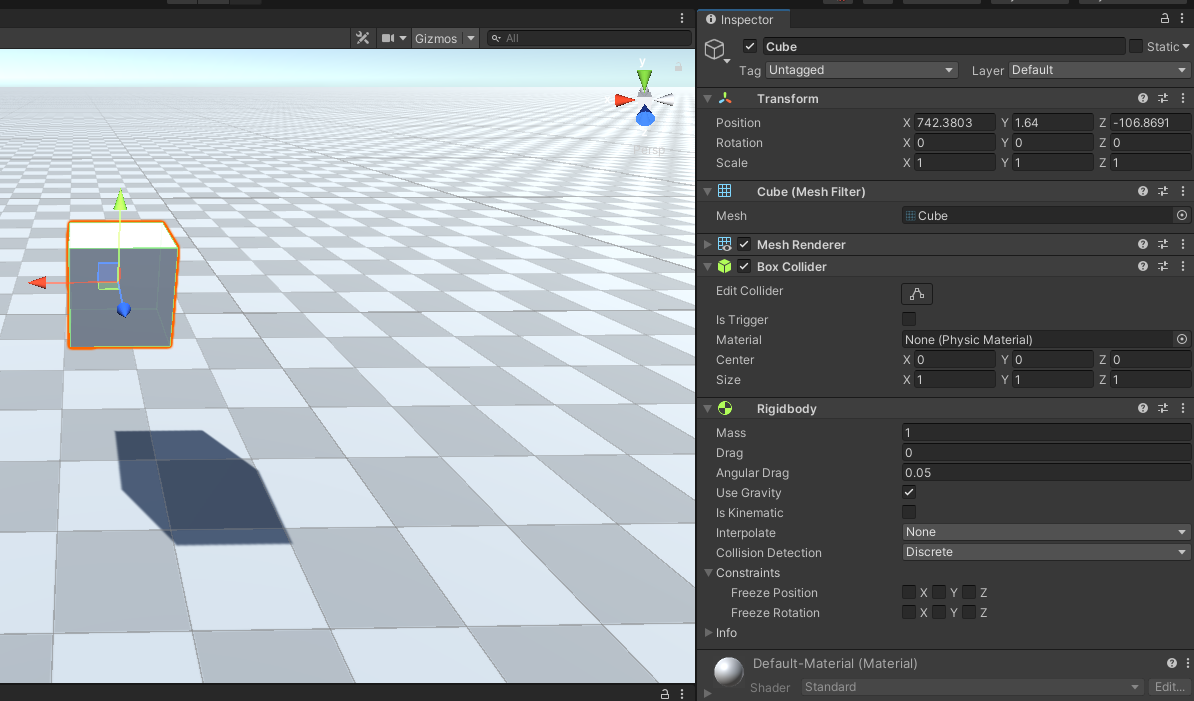
\includegraphics[width=0.8\linewidth]{"Immagini/RigidBody.png"}
		\caption{Questo è un cubo in unity, a destra possiamo vedere l'inspector con i component Box Collider e Rigidbody.}
		\label{fig:Rigidbody}
	\end{figure}
	Nella figura \ref{fig:Rigidbody} possiamo vedere un semplice cubo in \textsc{Unity} e sulla destra il suo Inspector. Il component \textsc{Collider} presenta parametri riguardo grandezza e posizione, e un campo \emph{"Is Trigger"} il quale indica che il collider è un \textsc{trigger}, cioè è attraversabile ed è possibile intercettare entrata, presenza all'interno e uscita di un oggetto. Mentre il \textsc{Rigidbody} presenta parametri per la massa, l'attrito e i vincoli sui movimenti e rotazione.
	\subsubsection{Telecamera}
	La camera in \textsc{Unity} è uno dei \textsc{GameObject} più importanti, essa presenta due \textsc{Component} principali:
	\begin{itemize}
		\item \textbf{Camera Component}, ciò che permette alla camera di riprendere il mondo di gioco
		\item \textbf{Audio Listener}, è il nostro "orecchio sul mondo di gioco" infatti ci permette di catturare i suoni prodotti dalle fonti sonore.
	\end{itemize}
	Il render della telecamera è gestito da una particolare figura geometrica chiamata \textsc{frustum}, nel caso specifico della telecamera è definito \textsc{frustum} di visione, il quale permette per l'appunto, di vedere quello che è presente in esso. Ogni parametro del \textsc{frustum} è modificabile nel \emph{Camera component}.
	\begin{figure}[H]
		\centering
		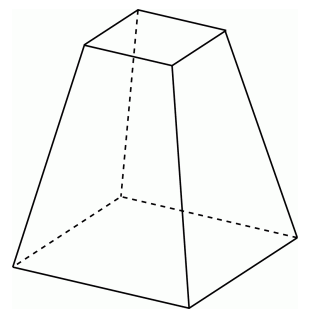
\includegraphics[width=0.5\linewidth]{"Immagini/frustum.png"}
		\caption{Questa è la figura geometrica frustum}
		\label{fig:frustum}
	\end{figure}
	\subsubitem{Particle System Shuriken}
		\textsc{Unity} presenta diversi sistemi di particelle, quello utilizzato per la simulazione è il \textsc{Particle System Shuriken}, il quale permette di gestire facilmente la collisione delle particelle. Il sistema di particelle permette di creare molti effetti tramite l'utilizzo di moduli per la gestione dei parametri.
		\begin{figure}[H]
			\centering
			\includegraphics[width=1\linewidth]{"Immagini/ParticleSystem"}
			\caption{Questi sono i moduli del Particle System Shuriken}
			\label{fig:ParticleSystem}
		\end{figure}
		La figura \ref{fig:ParticleSystem} mostra i diversi moduli  del \textsc{Particle System Shuriken}, ogni modulo presenta diversi parametri per modificare al meglio il sistema di particelle.
	\subsection{A* Pathfinding Project}
	\textsc{A* Pathfinding Project} \cite{A*} è un tool a cura di \emph{Aron Grandberg} che fa utilizzo del famoso algoritmo A* per il calcolo del percorso minimo.
		Ora introdurremo l'algoritmo per poi passare a descrivere nel dettaglio il tool.
		\textbf{A*} è un algoritmo di ricerca del tipo \emph{best-first} su grafi che individua un percorso da un nodo iniziale verso un nodo di destinazione. Ogni nodo ha un costo di entrata che rappresenta la distanza tra il nodo corrente e quello di inizio, e un valore che indica la distanza euristica dal nodo corrente a quello di destinazione, il costo del nodo è composto dalla somma dei due descritti precedentemente. L'algoritmo sceglie il nodo con costo totale minore, ricalcola il costo dei nodi vicini a quello scelto, continua così fino ad arrivare a destinazione.
		\begin{figure}[H]
			\centering
			\includegraphics[width=1\linewidth]{"Immagini/AStar"}
			\caption{Questo è un esempio dell'algoritmo su un grafo a griglia}
			\label{fig:AStar}
		\end{figure}
		Nella figura \ref{fig:AStar} possiamo vedere il percorso minimo calcolato con l'algoritmo A* in blu, in rosso possiamo vedere i nodi controllati, in verde quelli non controllati, mentre in nero abbiamo i nodi definiti come "ostacolo". 

		Ora andiamo nel dettaglio del tool di Aron Granberg. \\
		\textsc{A* pathfinding project} permette di scegliere tra diversi tipologie di grafi in modo tale da adattarlo ad ogni situazione. Le tipologie di grafi sono le seguenti:
		\begin{itemize}
			\item \textbf{Grafo a griglia}, come dice il nome è un grafo che genera nodi seguendo un pattern a griglia, è un pattern molto utile soprattutto quando bisogna aggiornare il grafo a runtime. Il grafo a griglia permette anche di scegliere la forma effettiva dei nodi, come ad esempio è possibile scegliere tra nodi quadrati, esagonali o personalizzati; oltre ad ovviamente permettere di scegliere quanti vicini ha ogni nodo.
			\item \textbf{Grafo Navmesh}, è un grafo che esprime i dati sul pathfinding come mesh a forma di triangolo. È un grafo che permette il calcolo del percorso minimo molto velocemente anche perché contiene meno nodi del grafo a griglia, quindi l'algoritmo richiede meno ricerca.
			\item \textbf{Grafo a punti}, è il più semplice tra tutti i tipi di grafi, permette una elevata personalizzazione e consiste in un gruppo di punti collegati tra loro.
		\end{itemize}
	Una volta scelto il grafo è possibile scegliere anche un \emph{layer} per indicare quali \textsc{GameObject} sono ostacoli in modo tale da evitarli.
	Per avere una personalizzazione completa del grafo è presente uno script, denominato \textsc{Graph Update Scene}, che permette di disegnare sul grafo delle aree e quindi impostare a piacimento i valori dei nodi di quell'area.
	Gli agenti che utilizzeranno il grafo per il calcolo del percorso minimo dovranno avere il due component principali, \textsc{AIPath}, il quale permette di impostare vari parametri, come la velocità dell'agente o l'accelerazione. \textsc{AIDestination Setter} il quale prende in input la destinazione dell'agente, il quale una volta impostata inizierà ad incamminarsi verso di essa. 
	
	\subsection{EasyRoad3D e Bézier Path Creator}
	\textsc{EasyRoad3D} \cite{EasyRoad3D} e \textsc{Bézier Path Creator} \cite{Bezier}
	sono due tool che si basano sulle curve di \textsc{Bézier}, delle curve formate da 4 punti: uno di inizio, uno di fine e due per la curvatura. \\
	\textsc{EasyRoad3d} permette, come si può intuire dal nome, creare facilmente delle strade su \textsc{Unity}. Il tool permette una grande personalizzazione delle strade, in più è tutto gestibile dall'inspector e dalla scena, infatti è possibile inserire dei punti per la creazione della strada con un semplice \textsc{shift+click}.\\
	\textsc{Bézier Path Creator} permette di disegnare un percorso tramite un insieme di punti e di modificare la curvatura del percorso seguendo le regole delle curve di \textsc{Bézier}. Sul percorso è possibile far muovere un \textsc{GameObject} facilmente assegnandogli lo script \textsc{Path follower}, il quale permette anche di impostare la velocità.
		\begin{figure}[H]
		\centering
		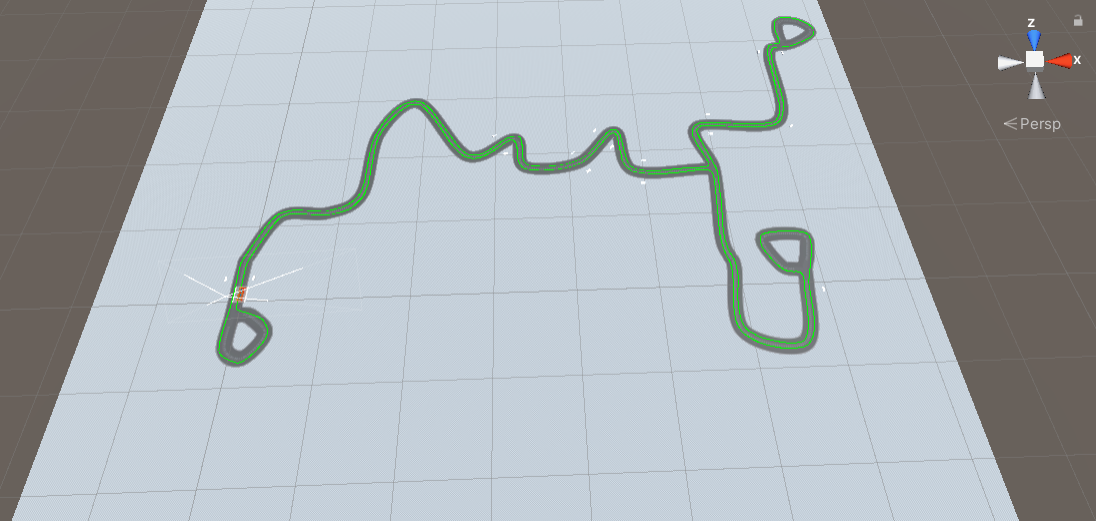
\includegraphics[width=1\linewidth]{"Immagini/EasyRoad+Bezier.png"}
		\caption{La strada creata con EasyRoad3D e il percorso creato con Beziér Path Creator}
		\label{fig:E+B}
	\end{figure}
	Nella Figura \ref{fig:E+B} è possibile vedere la strada realizzata con \textsc{EasyRoad3D} e, in verde è possibile vedere il percorso realizzato con \textsc{Beziér Path Creator}.
	
	\subsection{ProBuilder}
	\textsc{Probuilder} è un tool a cura di \textsc{Unity} stesso che permette di fare semplice modellazione direttamente in \textsc{Unity}, come è possibile vedere nella Figura \ref{fig:proBuilder}, esso infatti è stato utilizzato recentemente per lo sviluppo di alcuni videogiochi, come ad esempio \emph{SUPERHOT, Lucky's Tale, Tacoma}.\\
	Oltre a fornire diversi strumenti per la modellazione 3D, permette anche di generare delle forme predefinite come scale, archi e porte. È inoltre fornito di un'interfaccia grafica che si sovrappone alla scena in modo tale da avere tutti i tool a portata di click.
		\begin{figure}[H]
		\centering
		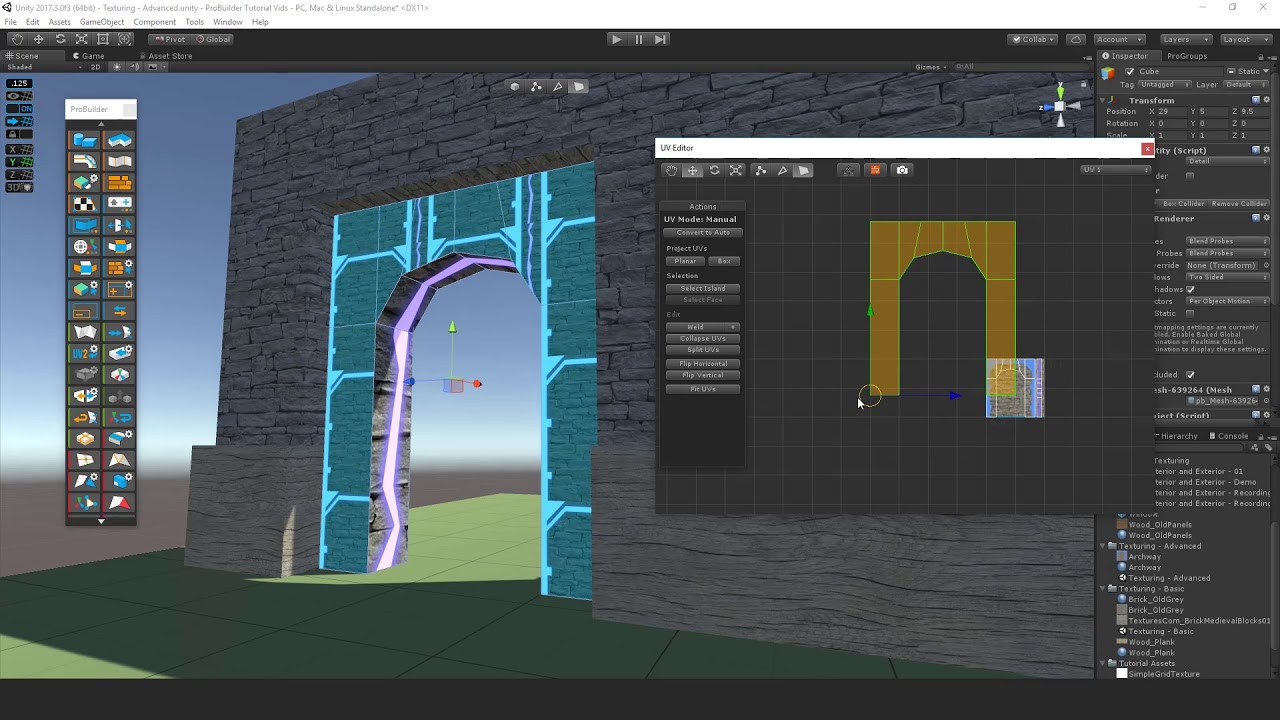
\includegraphics[width=1\linewidth]{"Immagini/probuilder.jpg"}
		\caption{Struttura modellata tramite ProBuilder}
		\label{fig:proBuilder}
	\end{figure}
	\subsection{Cinemachine}
	\textsc{Cinemachine} \cite{Cinemachine} è un tool a cura di \textsc{Unity} che permette di gestire con molta facilità e senza bisogno di scrivere codice la telecamera in \textsc{Unity}, ad esempio è possibile disegnare un percorso da far seguire alla telecamera. Il tool si basa sulla gestione di telecamere virtuali gestite da un \textsc{component} definito \textsc{Cinemachine brain}, dal quale è possibile passare da una camera all'altra e gestire le diverse inquadrature come è possibile vedere nella Figura \ref{fig:CinemachineLogo}. È possibile utilizzare anche una timeline per passare da una camera all'altra in un tempo specifico. Oltre ad essere stato utilizzato per la creazione di videogiochi, è stato utilizzato per la realizzazione di \emph{Baymax Dreams}, un'animazione in collaborazione con \emph{Disney Television Animation} con il quale hanno vinto un \emph{ Technology and Engineering Emmy Awards} il 7 aprile 2019.
		\begin{figure}[H]
		\centering
		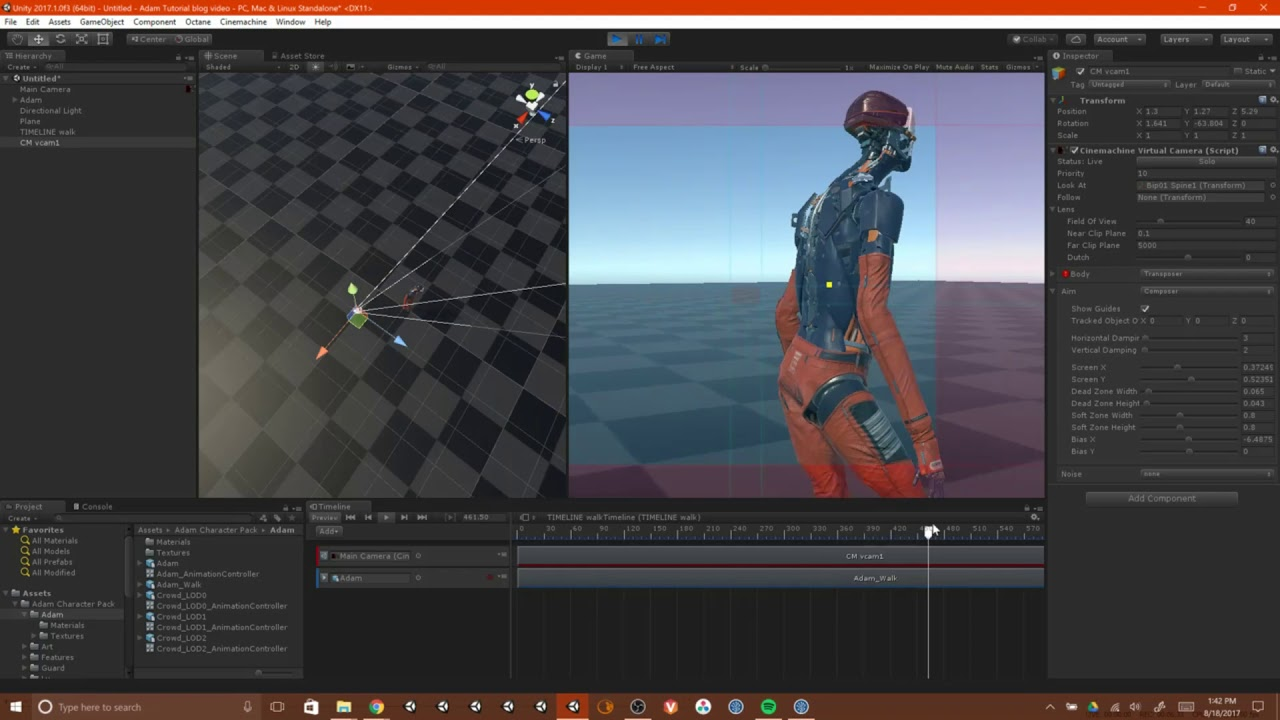
\includegraphics[width=1\linewidth]{"Immagini/CinemachineLogo.jpg"}
		\caption{Inquadratura realizzata con cinemachine}
		\label{fig:CinemachineLogo}
	\end{figure}
	
	
	\chapter{Simulazione}
	In questo capitolo si mostrerà il lavoro svolto nel dettaglio, per la realizzazione della simulazione. Partendo dalla simulazione base, per poi passare alla simulazione effettiva sulla strada di Obuse. 
	\section{La Strada di prova}
	Come prima cosa è stata realizzata una semplice strada circolare con \textsc{EasyRoad3D} in modo tale da poter mettere gli oggetti di scena e iniziare a fare delle prove.
	\begin{figure}[H]
		\centering
		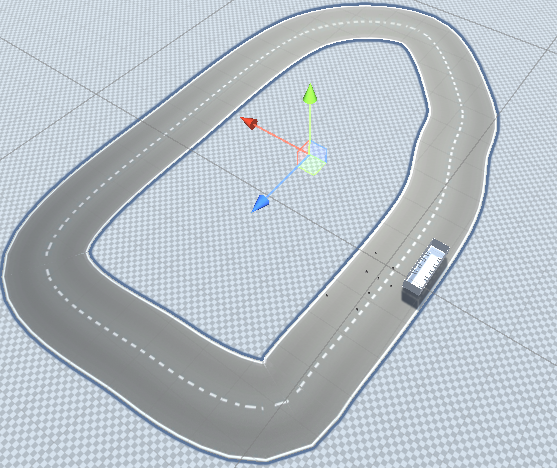
\includegraphics[width=0.7\linewidth]{"Immagini/StradaBase.png"}
		\caption{Questa è la strada di prova}
		\label{fig:StradaBase}
	\end{figure}
	Nella Figura \ref{fig:StradaBase} mostra la strada di prova utilizzata l'inizio della realizzazione della simulazione.\\
	Ora si parlerà dell'autobus, di come è stato creato ed utilizzato e di come ce ne siano state diverse versioni. 
	\begin{figure}[H]
		\centering
		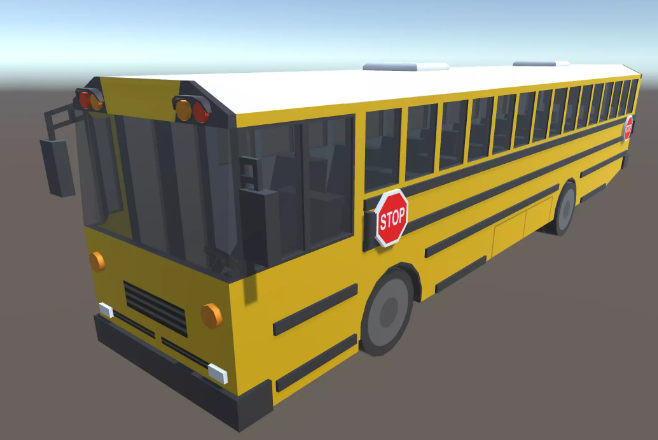
\includegraphics[width=0.7\linewidth]{"Immagini/SchoolBus.png"}
		\caption{Questo è stato il primo bus della simulazione}
		\label{fig:SchoolBus}
	\end{figure}
	\section{Il mezzo di trasporto}
	L'autobus è stato realizzato con \textsc{ProBuilder}, esso presenta 12 posti, i quali a loro volta hanno un target ognuno. Per facilitare la salita degli agenti è presente una rampa che compare solo nel momento in cui il bus è fermo.
		\begin{figure}[H]
		\centering
		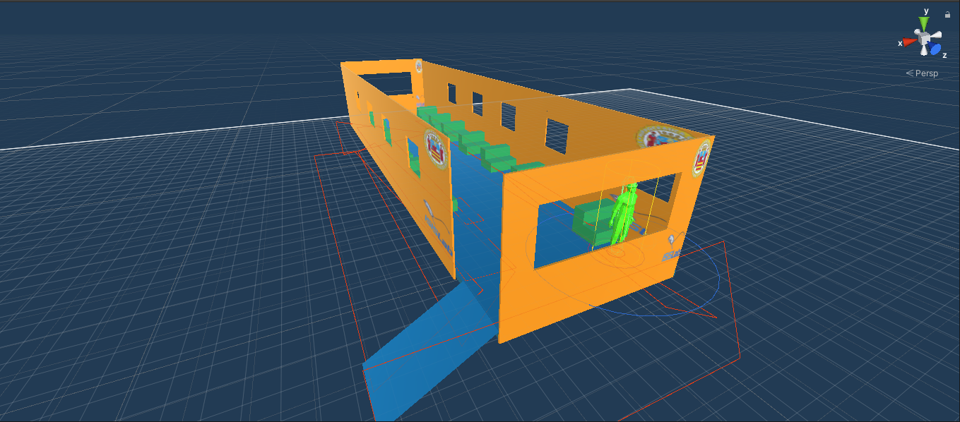
\includegraphics[width=1\linewidth]{"Immagini/BusComplete.png"}
		\caption{Il bus finale}
		\label{fig:busFinale}
	\end{figure}
	\section{L'agente}
	 Si è poi passati all'inserimento dei modelli degli agenti e quindi a lavorare sulle varie animazioni. 
	\section{Il percorso del mezzo di trasporto}
	Come è possibile vedere dallo script \ref{SitDown} alla riga 14 viene risolto il problema dell'agente al di sotto del bus riposizionandolo nella giusta posizione.\\
	Si è poi passati all'integrazione del tool \emph{Beziér Path Creator}, per far muovere l'autobus. Quindi si è tracciato un percorso sulla strada in modo tale che il bus lo seguisse.
	\begin{figure}[H]
		\centering
		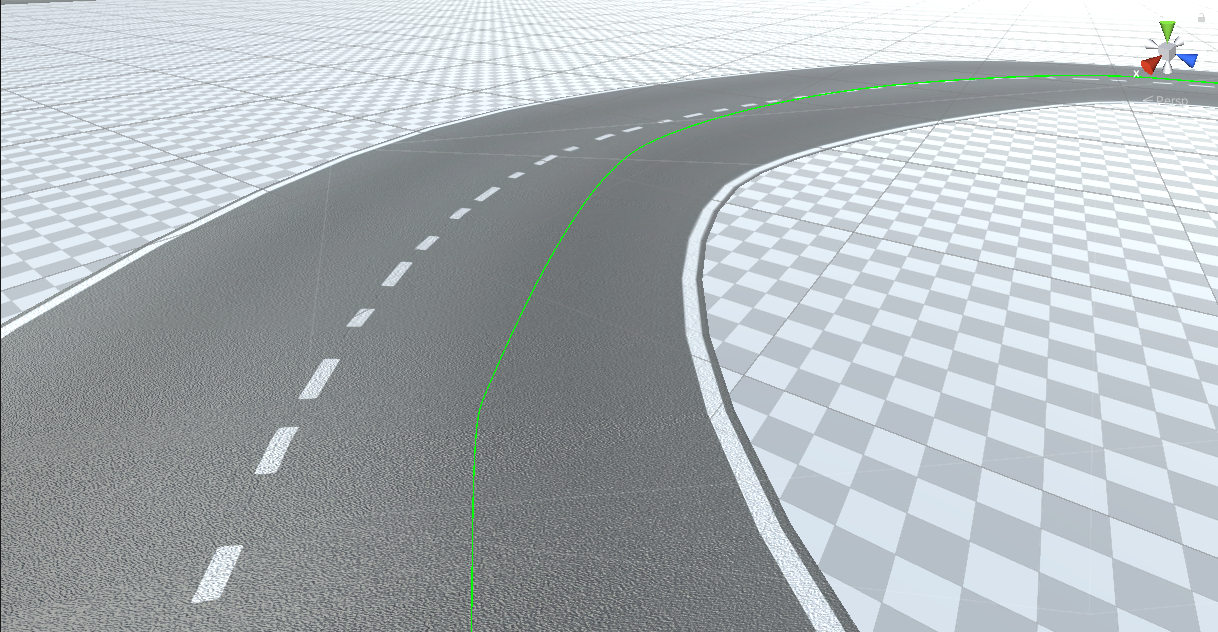
\includegraphics[width=1\linewidth]{"Immagini/BezierPath.png"}
		\caption{Questo è un tratto del percorso.}
		\label{fig:BezierPath}
	\end{figure}
	Nella Figura \ref{fig:BezierPath} si vede, in verde, un tratto del percorso disegnato con \textsc{Beziér Path Creator} sul quale il bus si muove.\\

	\section{La fermata}
	Giunti alla situazione nella quale gli agenti salgono correttamente sul bus, prendono posto e si siedono, il bus si muove seguendo il percorso disegnato ci si è spostati sulla creazione di fermate per gli agenti, in modo tale da simulare le varie tratte dell'autobus, iniziando con una semplice struttura e una linea che funge da \textsc{trigger} per far si che l'autobus si fermi.\\
	\begin{figure}[H]
		\centering
		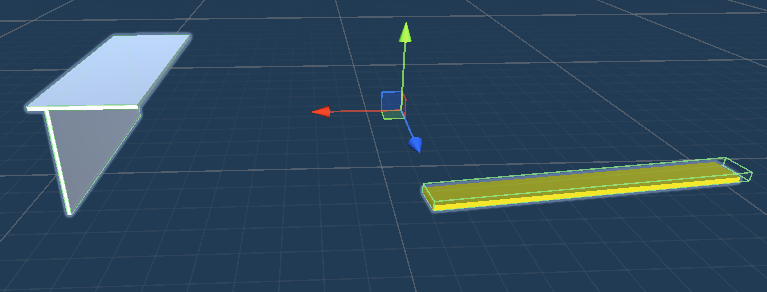
\includegraphics[width=1\linewidth]{"Immagini/BusStopNoSA.png"}
		\caption{Fermata del bus}
		\label{fig:BusStopNoSA}
	\end{figure}
	Nella Figura \ref{fig:BusStopNoSA} è possibile vedere una semplice struttura per dare l'idea di fermata, sulla sinistra, mentre sulla destra abbiamo la linea che fa da \textsc{trigger} per l'autobus.\\
	
	 È stato poi considerato utile aggiungere un \textsc{GameObject} denominato \textsc{Spawning Area}, all'interno di ciascuna fermata con il quale era possibile impostare la grandezza dell'area dove venivano generati gli agenti, deciderne il numero e decidere la velocità di ripartenza del bus. Questa scelta si è rivelata molto utile per passare dalla scena di prova a quella effettiva della simulazione.
	 \begin{figure}[H]
	 	\centering
	 	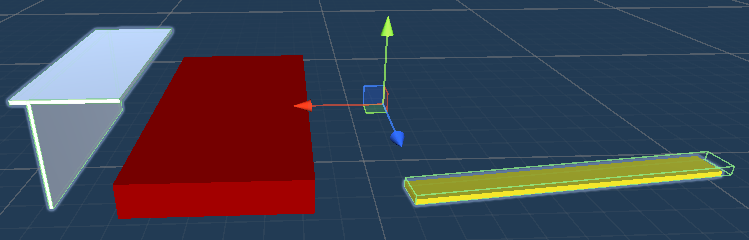
\includegraphics[width=1\linewidth]{"Immagini/BusStopSA.png"}
	 	\caption{Fermata del bus con area di spawning}
	 	\label{fig:BusStopSA}
	 \end{figure}
 	L'area rossa nella Figura \ref{fig:BusStopSA} è l'area di spawning, nella quale vengono generati gli agenti, di seguito nella Figura \ref{fig:SAInspector} verrà mostrato nel dettaglio l'inspector dell'area.
 	\begin{figure}[H]
 		\centering
 		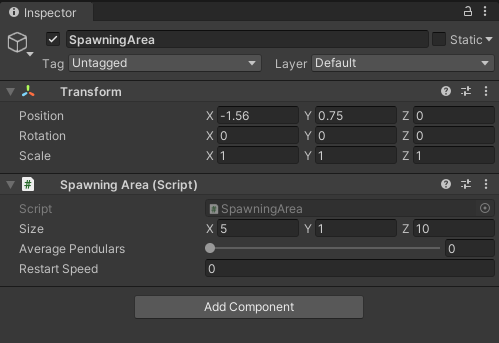
\includegraphics[width=1\linewidth]{"Immagini/SAInspector.png"}
 		\caption{Inspector dell'area di spawning}
 		\label{fig:SAInspector}
 	\end{figure}
 	Tramite la variabile \textsc{Size} è possibile modificare l'area nella quale verranno generati gli agenti; \textsc{Average Pendulars} permette di impostare il numero medio di agenti da generare alla fermata, il perché del numero medio di agenti invece di un numero fisso verrà spiegato in seguito; \textsc{Restart Speed} permette di decidere la velocità di ripartenza del bus in modo tale da poter far rispettare degli orari reali.  
 	\section{Il GameControl}
 		Il \textsc{GameControl} è il \textsc{GameObject} che gestisce buona parte dei parametri della simulazione,  infatti esso gestisce la generazione degli agenti, quanti agenti sono contagiosi all'interno della simulazione, la percentuale di che un agente venga infettato da una singola particella o il calcolare le statistiche della simulazione e scriverle su file.
 		\begin{figure}[H]
 			\centering
 			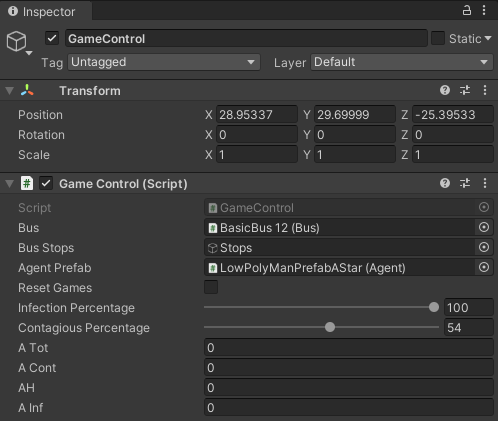
\includegraphics[width=1\linewidth]{"Immagini/GameControl.png"}
 			\caption{L'inspector del GameControl}
 			\label{fig:GameControl}
 		\end{figure}
 		Nella Figura \ref{fig:GameControl} è possibile vedere i parametri dell'oggetto GameControl citati precedentemente.
 	\section{La tratta di Obuse}
 	Con la simulazione funzionante si è poi passati alla ricerca di documenti su tratte di autobus reali, trovando un articolo riguardo al volume dei passeggeri sulla tratta di bus della cittadina giapponese Obuse  \cite{Obuse}, il volume è stato calcolato tramite una stima basata sui Wi-Fi scanner presenti sulla tratta.
 	\begin{figure}[H]
 		\centering
 		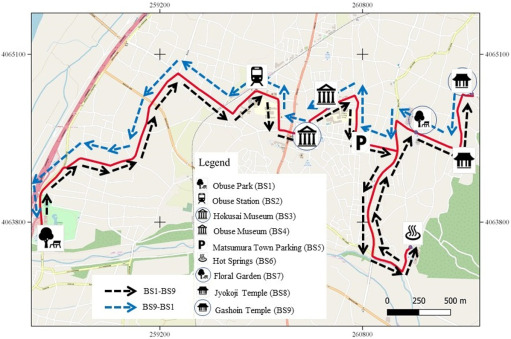
\includegraphics[width=1\linewidth]{"Immagini/MappaObuse.jpg"}
 		\caption{Mappa della tratta di Obuse}
 		\label{fig:Map}
 	\end{figure}
 	Nella Figura \ref{fig:Map} si vede, in rosso, la tratta del bus, mentre nella Figura \ref{fig:Pendolari} si vede la media dei pendolari su ogni fermata della tratta.
 	\begin{figure}[H]
 		\centering
 		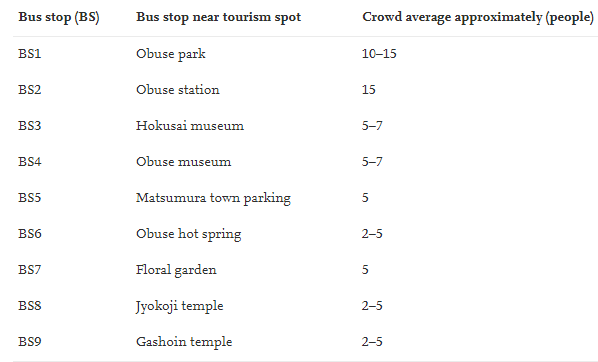
\includegraphics[width=1\linewidth]{"Immagini/MediaPendolari.png"}
 		\caption{Media di pendolari per ogni fermata della tratta}
 		\label{fig:Pendolari}
 	\end{figure}
 	Considerando che i dati sono stati raccolti prima della pandemia da \textsc{CoViD-19}, è stato deciso di dimezzare i dati. Si è passati quindi dal bus a 24 posti ad uno a 12 posti, si è dimezzato il numero di pendolari per ogni fermata, e si è deciso di generare un numero di pendolari in un intervallo di $\pm30\%$ della media calcolata tramite \textsc{Wi-Fi} scanner.
 	\begin{lstlisting}[language={[Sharp]C}, 
 		caption={Genera i pendolari alle fermate}, label={SpawningAtStops}]
 		   public void SpawningAtStops()
 		{
 			
 			List<SpawningArea> areas = new List<SpawningArea>();
 			foreach (Transform stop in stops)
 			{
 				List<SpawningArea> spawnAreas=Utility<SpawningArea>.GetAllChildren(stop.gameObject);
 				areas.Add(spawnAreas[0]);
 				areas.Add(spawnAreas[1]);
 				
 			}
 			foreach (SpawningArea area in areas)
 			{
 				
 				int effectivePendulars = Random.Range(area.AvaragePendulars - area.AvaragePendulars * 30 / 100, area.AvaragePendulars + area.AvaragePendulars * 30 / 100);
 				
 				for (int i = 0; i < effectivePendulars; i++)
 				SpawnAgent(area);
 			}
 		}
 	\end{lstlisting}
 	Nel Script \ref{SpawningAtStops}, alla riga 15, è presente il codice che indica il range di $\pm30\%$ della media.\\
 	Si è poi passati alla realizzazione in scala della strada su Unity utilizzando \textsc{EasyRoad3D} come è si vede nella Figura \ref{fig:ObuseStreet}, in verde è possibile anche vedere il percorso del bus realizzato con \textsc{Bezièr Path Creator}. 
 	\begin{figure}[H]
 		\centering
 		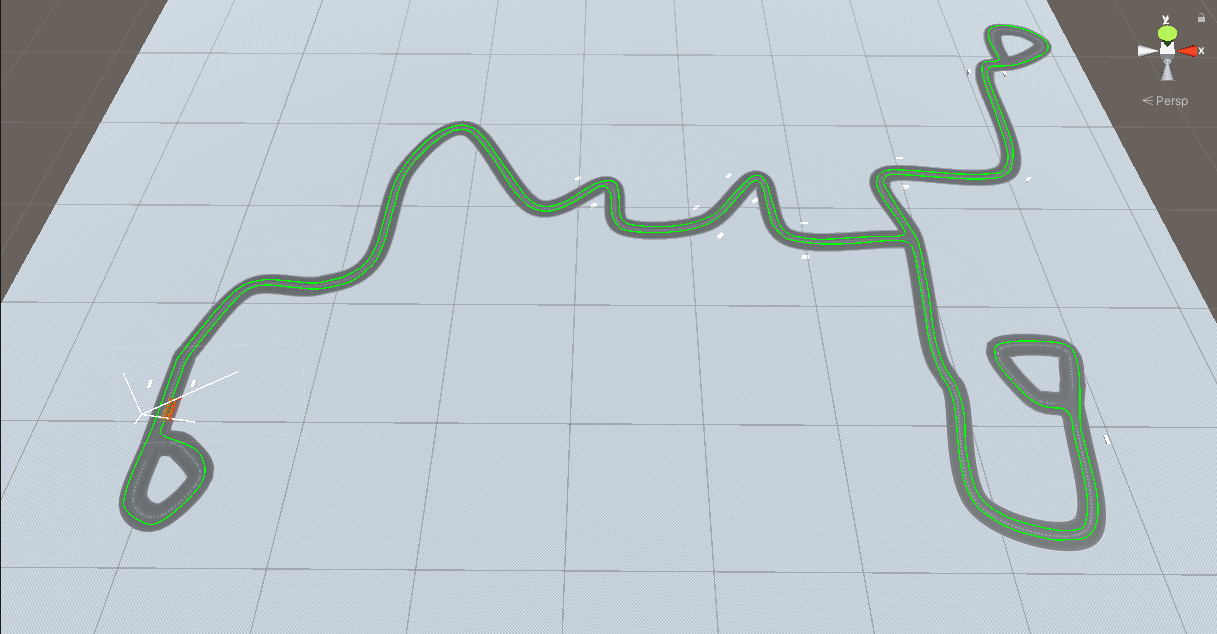
\includegraphics[width=1\linewidth]{"Immagini/ObuseStreet.png"}
 		\caption{Strada di Obuse in Unity}
 		\label{fig:ObuseStreet}
 	\end{figure}
 
 
 	\section{La telecamera}
 	La telecamera è stata gestita completamente con il tool \textsc{Cinemachine}, come è possibile vedere nella Figura \ref{fig:Cinemachine}, il quale ha permesso di creare una telecamera isometrica che seguisse il bus per l'intera simulazione senza scrivere codice.
 	\begin{figure}[H]
 		\centering
 		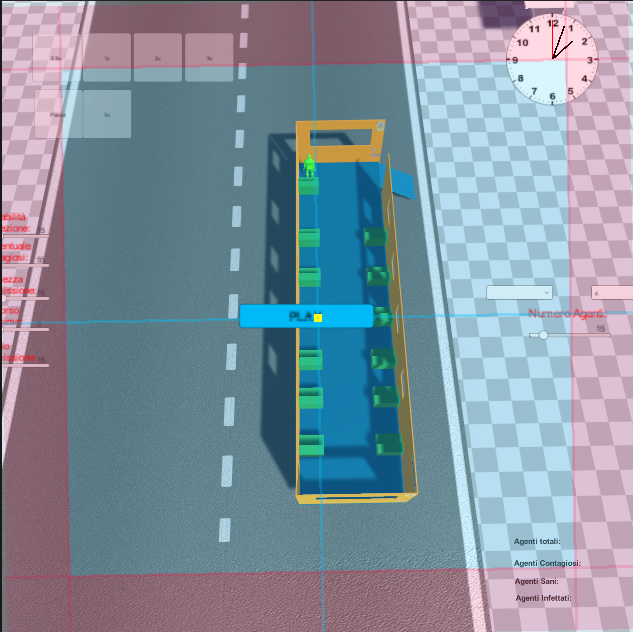
\includegraphics[width=0.7\linewidth]{"Immagini/Cinemachine.png"}
 		\caption{La griglia della telecamera, il puntino giallo indica l'oggetto da seguire}
 		\label{fig:Cinemachine}
 	\end{figure}


\chapter{Simulazione degli agenti}
	In questo capitolo si parlerà nel dettaglio degli agenti, della sezione di contagio e interfaccia grafica. Gli agenti all'interno, della simulazione presentano tre stati: \textbf{Sano, Infetto e Contagioso}.
	\section{Gli stati degli agenti}
	Un agente \textbf{Sano} è denotato da un colore della \textsc{texture} verde come è possibile vedere nella Figura \ref{fig:agenteSano}. Un agente \textbf{sano} è caratterizzato dalla presenza di un collider, il quale permette all'agente di infettarsi nel caso di un contatto con una particella di \textsc{CoViD-19}.	
	\begin{figure}[H]
		\centering
		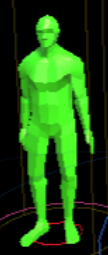
\includegraphics[width=0.1\linewidth]{"Immagini/AgenteSano.png"}
		\caption{Agente Sano}
		\label{fig:agenteSano}
	\end{figure}.
	Un agente \textbf{Infetto} è un agente che è stato infettato da una particella di \textsc{CoViD-19} ed è denotato da un colore della \textsc{texture} giallo come è possibile vedere nella Figura \ref{fig:agenteInfetto}. L'agente \textbf{infetto} sta ad indicare la fase di incubazione del \textsc{CoViD-19}, la quale può durare fino a due settimane. In questa fase l'agente non può contagiarne altri. Data la durata dell'incubazione all'interno della simulazione non è possibile vedere quindi il cambiamento di stato dell'agente da \textbf{infetto} a \textbf{contagioso}, ovviamente perché, la durata della tratta è di poche ore.	\begin{figure}[H]
		\centering
		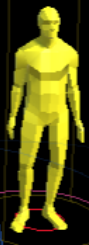
\includegraphics[width=0.1\linewidth]{"Immagini/AgenteInfetto.png"}
		\caption{Agente Infetto}
		\label{fig:agenteInfetto}
	\end{figure}.
	Un agente \textbf{Contagioso}, infine, è un agente che può infettare altri agenti. É denotato da un colore della \textsc{texture} rosso come è possibile vedere della Figura \ref{fig:agenteContagioso} Esso emette delle particelle di \textsc{CoViD-19}, per simulare i colpi di tosse, le quali, entrando in contatto con il collider di un agente \textbf{Sano} possono farlo passare allo stato di \textbf{Infetto}	
	\begin{figure}[H]
		\centering
		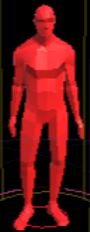
\includegraphics[width=0.1\linewidth]{"Immagini/AgenteContagioso.png"}
		\caption{Agente Contagioso}[r]
		\label{fig:agenteContagioso}
	\end{figure}.
	\pagebreak
	\section{Comportamento degli agenti}
	Gli agenti sono dotati di un set di quattro animazioni:
	\begin{itemize}
		\item \textbf{Attesa}
		\item \textbf{Camminata}
		\item \textbf{Seduta}
		\item \textbf{Alzata}
	\end{itemize}
		\begin{figure}[H]
		\centering
		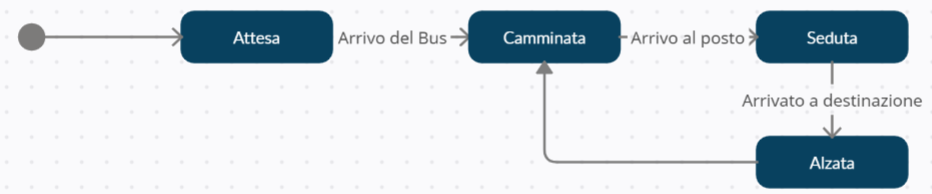
\includegraphics[width=1\linewidth]{"Immagini/StatiAnimazioni.png"}
		\caption{Comportamento dell'agente}
		
		\label{fig:StatiAnimazioni}
			\end{figure}
		Nella Figura \ref{fig:StatiAnimazioni} c'è la rappresentazione della macchina a stati. Un agente di \textsc{default} è nello stato di \textsc{Attesa}, una volta che il bus arriva alla fermata e l'agente può salire, entra nello stato di \textsc{Camminata} per poi entrare nello stato di \textsc{Seduta}. Una volta che il bus è arrivato alla fermata di destinazione dell'agente, esso entra nello stato di \textsc{Alzata} per poi passare immediatamente nello stato di \textsc{Camminata} per uscire dal bus.


\begin{figure}
	\centering
	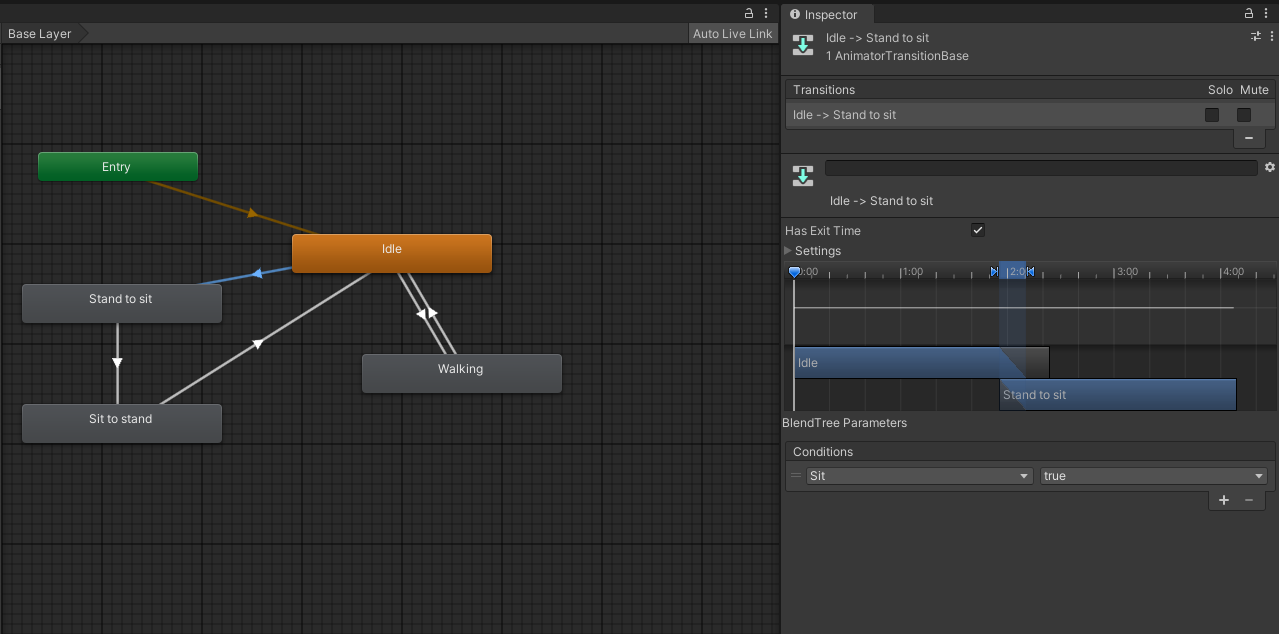
\includegraphics[width=1.2\linewidth]{"Immagini/AgentAnimator.png"}
	\caption{Questo è il component animator dell'agente}
	\label{fig:AgentAnimator}
\end{figure}
La Figura \ref{fig:AgentAnimator} mostra sulla sinistra la macchina a stati finiti composta dagli stati in cui si può trovare l'agente, ogni stato ha la sua animazione. Sulla destra invece possiamo vedere una prospettiva sulla transizione che va dallo stato di \emph{idle} a quello di \emph{Stand to Sit}, come si può vedere in basso la transizione avviene quando la variabile booleana Sit ha valore pari a true.\\
\begin{figure}[H]
	\centering
	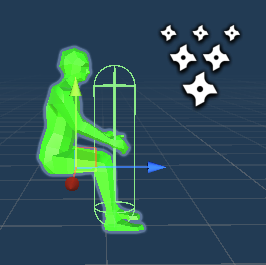
\includegraphics[width=0.8\linewidth]{"Immagini/seduto.png"}
	\caption{Frame dell'animazione di seduta}
	\label{fig:Seduta}
\end{figure}
Nella Figura \ref{fig:Seduta} è mostrato un frame dell'animazione di seduta e il collider dell'agente che si restringe.
\begin{figure}[H]
	\centering
	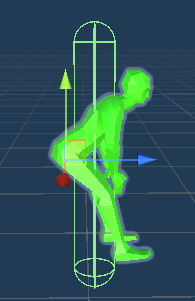
\includegraphics[width=0.8\linewidth]{"Immagini/inPiedi.png"}
	\caption{Frame dell'animazione di alzata}
	\label{fig:Alzata}
\end{figure}
Nella Figura \ref{fig:Alzata} si può vedere un frame dell'animazione di alzata, denominata \emph{Sit to Stand}, si può vedere anche il collider dell'agente che ritorna alla forma originale.\\
Il passaggio delle varie animazioni è stato gestito da script assegnando valore alle variabili booleane dell'\textsc{animator}.
\begin{lstlisting}[language={[Sharp]C}, 
	caption={Metodo che permette agli agenti di prendere posto sull'autobus}, label={TakeBus}]
	public void TakeBus()
	{
		if (!bus.isMooving && bus.FreeTarget() != null && target== null)
		{
			animator.SetBool("Waiting", false);
			target = bus.FreeTarget();
			SetDestination(target);
		}
	}
\end{lstlisting}	
Lo script \ref{TakeBus} è il metodo all'interno della classe \textsc{Agent} con il quale l'agente prende un posto a sedere sul bus, rendendolo occupato ed inizia ad incamminarsi verso di esso. Come è possibile vedere dalla riga 5, si modifica la variabile booleana \textsc{Waiting}, all'interno del component \textsc{Animator} assegnandole valore pari a \emph{false} così da passare dallo stato di \textsc{Waiting} allo stato di \textsc{Walking} .  \newpage
A questo punto della simulazione gli agenti si sedevano correttamente, ma spesso capitava che facessero percorsi strani o che camminassero sopra i posti a sedere, per questo motivo al bus sono stati aggiunti diversi \textsc{GameObject} con component \textsc{Graph Update Scene}, in modo tale da poter penalizzare dei nodi del grafo per avere un percorso migliore per gli agenti.
\begin{figure}[H]
	\centering
	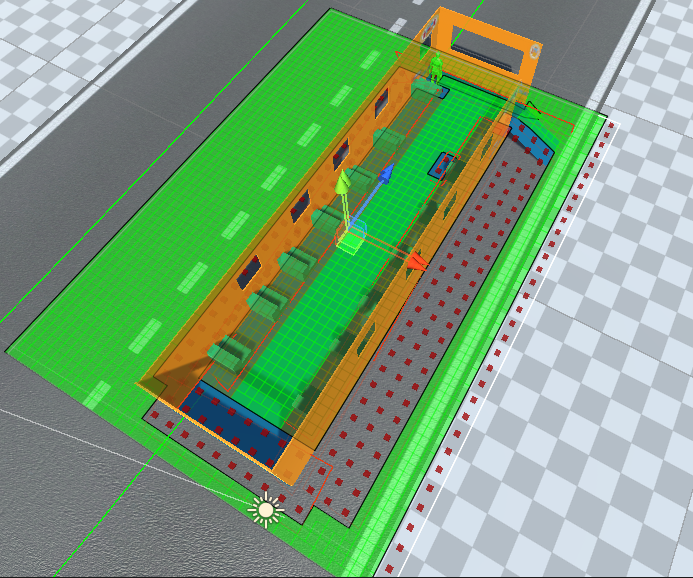
\includegraphics[width=1\linewidth]{"Immagini/AreaGrafo.png"}
	\caption{Questo è il grafo definitivo della simulazione.}
	\label{fig:AreaGrafo}
\end{figure}
Nella Figura \ref{fig:AreaGrafo} possiamo vedere diverse zone nel grafo: le zone verdi sono aree completamente calpestabili, quindi non modificate dal \textsc{Graph Update Scene}; Le aree rosse sono aree calpestabili ma con penalità, per evitare che gli agenti scavalchino i sedili; le zone trasparenti con quadrati rossi sono zone non calpestabili. In più si può vedere il bus finale che è stato utilizzato nella simulazione definitiva di Obuse a 12 posti, in seguito se ne parlerà più approfonditamente.
In seguito si è passati all'integrare il \textsc{local avoidance} tramite \textsc{Reciprocal Velocity Obstacles (RVO)} del tool \textsc{A* Pathfinding Project}, il quale ha permesse di gestire facilmente il distanziamento tra gli agenti, impedendo compenetrazioni e varie problematiche che potevano accadere implementando tale funzione. Un problema però è presente, alla salita degli agenti sul bus può capitare che distanziandosi sulla rampa, gli agenti cadano da essa finendo col camminare al di sotto del bus. Questo è stato risolto riposizionando, una volta arrivati a destinazione, gli agenti sul posto assegnato.

\begin{lstlisting}[language={[Sharp]C}, caption={Metodo per la seduta degli agenti}, label={SitDown}]
	private void SitDown()
	{
		if (State == States.Healthy)
		{
			gameObject.AddComponent<ColliderCovid>();
			GetComponent<ColliderCovid>().InfectionPercentage = 	gameControl.infectionPercentage;
		}
		StartCoroutine(RotateOnSpot());
		aiPath.enabled = false;
		animator.SetBool("Waiting", true);
		animator.SetBool("Sit", true);
		rigidCube.tag = "Exiting";
		
		transform.position = target.transform.position;
		bool haveRigidBody = gameObject.GetComponent<Rigidbody>() != null;
		
		if (!haveRigidBody)
		{
			gameObject.AddComponent<Rigidbody>().freezeRotation = true;
		}
	}
\end{lstlisting}

 	\section{Il virus}
La diffusione del virus è stata gestita tramite il \textsc{particle system shuriken} di \textsc{Unity}, il quale permette di gestire facilmente le collisioni con le particelle. Si è iniziati a realizzare un \textsc{particle system} che desse l'effetto dello spostamento d'aria, quindi un effetto di fumo che uscisse dalla bocca come è possibile vedere nella Figura \ref{fig:SmokeEffect}.
\begin{figure}[H]
	\centering
	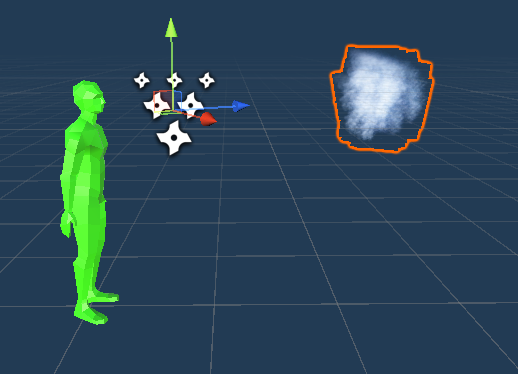
\includegraphics[width=0.5\linewidth]{"Immagini/SmokeEffect.png"}
	\caption{Effetto di fumo che parte dalla bocca dell'agente}
	\label{fig:SmokeEffect}
\end{figure}
Quindi si è passati alla realizzazione di un \textsc{particle system} che avesse un collider sulle particelle, un semplice effetto con delle sfere, inizialmente formate da un modello di \textsc{CoViD-19} visibile nella Figura \ref{fig:Covid}
\begin{figure}[H]
	\centering
	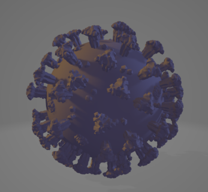
\includegraphics[width=0.5\linewidth]{"Immagini/Covid.png"}
	\caption{Modello dettagliato di CoViD-19}
	\label{fig:Covid}
\end{figure}
Per poi essere sostituito per ottimizzazione delle performance in seguito, ma questo se ne parlerà nella sezione dell'ottimizzazione.
\begin{figure}[H]
	\centering
	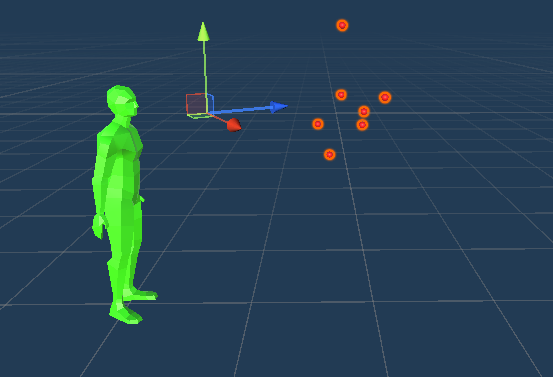
\includegraphics[width=0.5\linewidth]{"Immagini/CovidEffect.png"}
	\caption{Effetto che simula le particelle infette di \textsc{CoViD-19} in un colpo di tosse}
	\label{fig:CovidEffect}
\end{figure}
Nella Figura \ref{fig:CovidEffect} si vede l'effetto delle particelle che simulano quelle infette da \textsc{CoViD-19}, ogni particella ha un collider che permette di catturare le collisioni con il \textsc{collider} dell'agente sano che è possibile vedere nella Figura \ref{fig:ColliderCovid}
\begin{figure}[H]
	\centering
	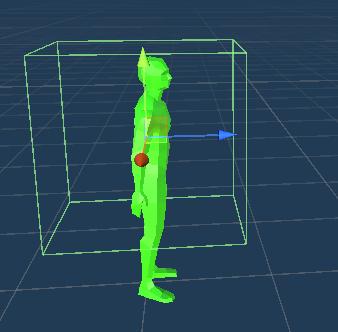
\includegraphics[width=0.5\linewidth]{"Immagini/ColliderCovid.png"}
	\caption{Il collider con il quale l'agente può essere infettato da una particella}
	\label{fig:ColliderCovid}
\end{figure}
Una volta che una particella di \textsc{CoViD-19} entra in collisione con il \textsc{collider} dell'agente sano, esso può diventare infetto, e quindi cambiare colore da verde a giallo


	\section{L'interfaccia}
Una volta arrivati alla simulazione funzionante, si è passati alla realizzazione di un'interfaccia grafica semplice ed intuitiva, inserendo l'orologio che scandisce il tempo reale, degli slider per la gestione dei parametri, dei pulsanti per la gestione del tempo della simulazione e del testo per i dati sul contagio. L'interfaccia grafica si divide in due parti, quando la simulazione è in pausa e quando è in play.
\begin{figure}[H]
	\centering
	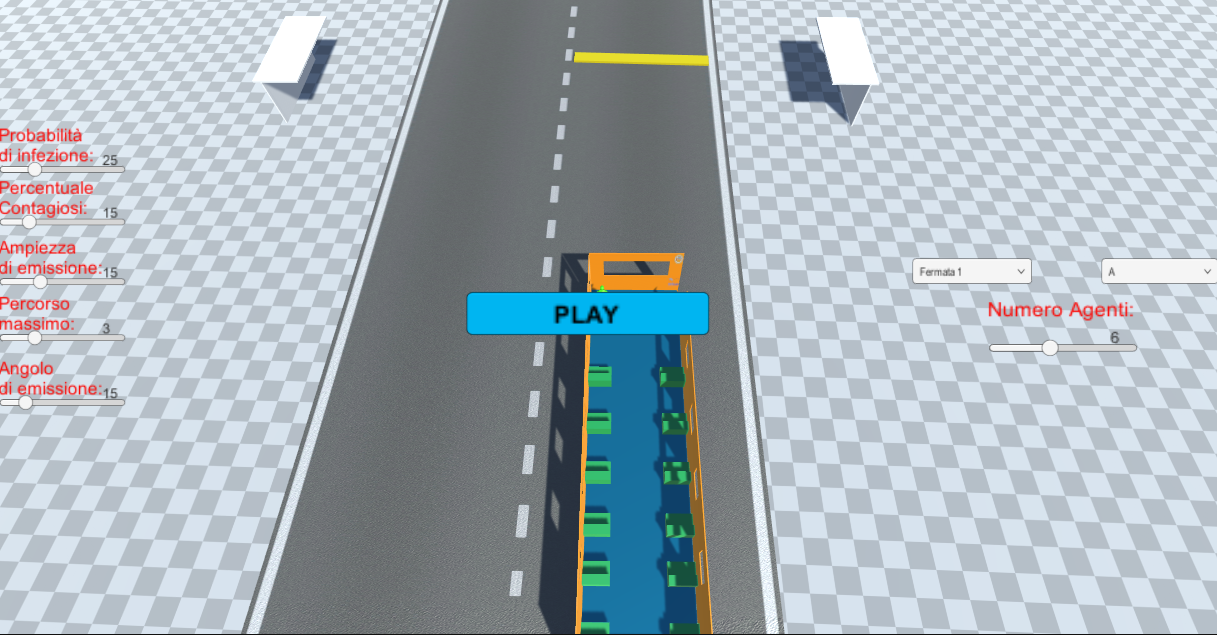
\includegraphics[width=0.8\linewidth]{"Immagini/PausedGui.png"}
	\caption{Interfaccia della simulazione in pausa}
	\label{fig:InterfacciaPausa}
\end{figure}
Nella Figura \ref{fig:InterfacciaPausa} sono presenti diversi \textsc{slider}, sulla sinistra per la gestione dei parametri di contagio, sulla destra sono presenti due menù tendina e uno \textsc{slider} per scegliere il numero di agenti da generare su una fermata selezionata dai menù, infine un pulsante al centro per far partire la simulazione.
Ora parliamo più nel dettaglio degli elementi presenti nell'interfaccia:\\
\begin{itemize}
	\item Probabilità di infezione, permette di modificare la probabilità che ha una particella di infettare un agente quando vi entra in contatto.
	\item Percentuale Contagiosi, permette di modificare percentuale di contagiosi che vengono generati ad ogni tratta.
	\item Ampiezza di emissione, permette di modificare l'ampiezza del cono di emissione delle particelle.
	\item Percorso minimo, permette di modificare la tratta massima, in numero di fermate, che un agente percorrerà sull'autobus.
	\item Angolo di emissione, permette di modificare l'intervallo dell'angolo del cono di emissione.
	\item Numero Agenti, permette di scegliere il numero di agenti nella fermata scelta dal menù a tendina.
	\item Il tasto \emph{PLAY} serve ad avviare la simulazione.
\end{itemize}

\begin{figure}[H]
	\centering
	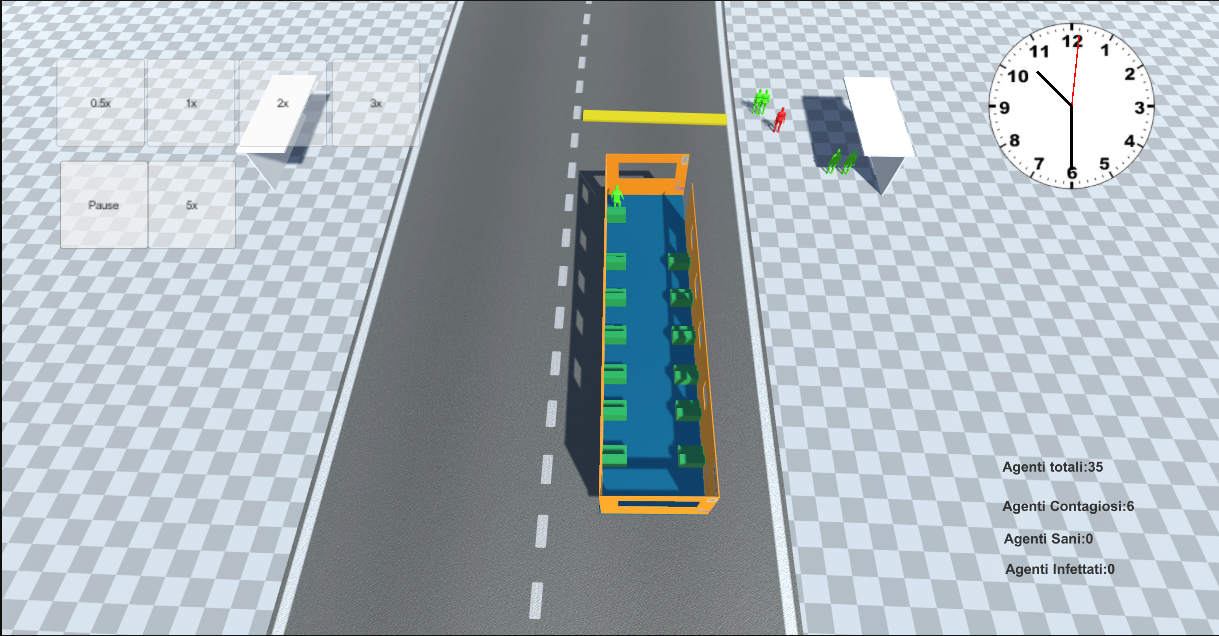
\includegraphics[width=0.8\linewidth]{"Immagini/PlayGui.png"}
	\caption{Interfaccia della simulazione in play}
	\label{fig:InterfacciaPlay}
\end{figure}
Nella Figura \ref{fig:InterfacciaPlay} sono presenti, sulla sinistra i bottoni per la gestione del tempo, in alto a destra un orologio che scandisce il tempo reale della simulazione e in basso a destra sono presenti i dati del contagio della simulazione.
		\section{La raccolta dei dati}
	La raccolta dei dati avviene tramite una scrittura su file \textsc{csv}. Ad ogni avvio della simulazione viene generato un file contenente le informazioni riguardo il contagio, come è possibile vedere nella Figura \ref{fig:csv}. Ad ogni tratta viene generata una riga contenente il numero di agenti totali, quelli contagiosi, quelli infetti e quelli sani.
	\begin{figure}[H]
		\centering
		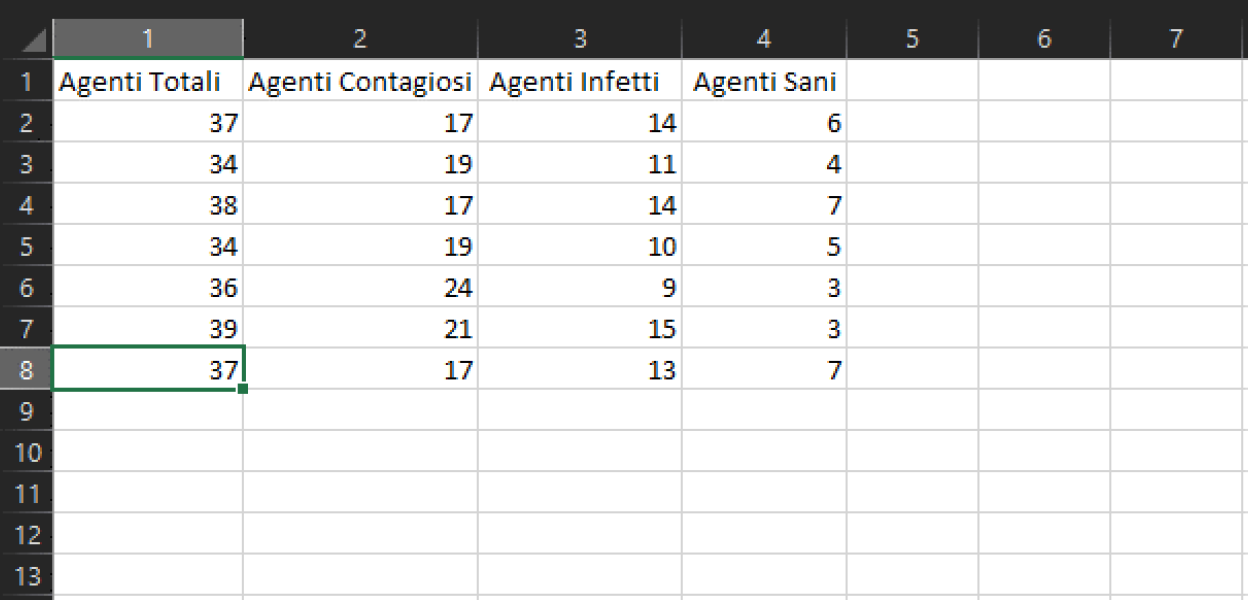
\includegraphics[width=1\linewidth]{"Immagini/csv.png"}
		\caption{Raccolta dati di una simulazione completa}
		\label{fig:csv}
	\end{figure}
	Il conteggio degli agenti totali e di quelli contagiosi avviene alla loro generazione; quelli infetti vengono conteggiati appena vengono infettati da una particella; quelli sani vengono conteggiati appena scendono dal bus.
 	\section{L'ottimizzazione}
Il lavoro di ottimizzazione è iniziato nel momento in cui la simulazione aveva cali drastici di \textsc{framerate}, anche su diverse macchine. Tramite il  \textsc{Profiler}, strumento presente in \textsc{Unity} in grado di mostrare l'utilizzo di risorse della macchina e quale processo in particolare sta sfruttando le risorse, si è riusciti a comprendere quali erano i principali problemi. Come è possibile vedere dalla Figura \ref{fig:ProfilerFPSBassi} ci sono dei cali drastici a 15 \textsc{FPS} che causano non pochi problemi.
\begin{figure}[H]
	\centering
	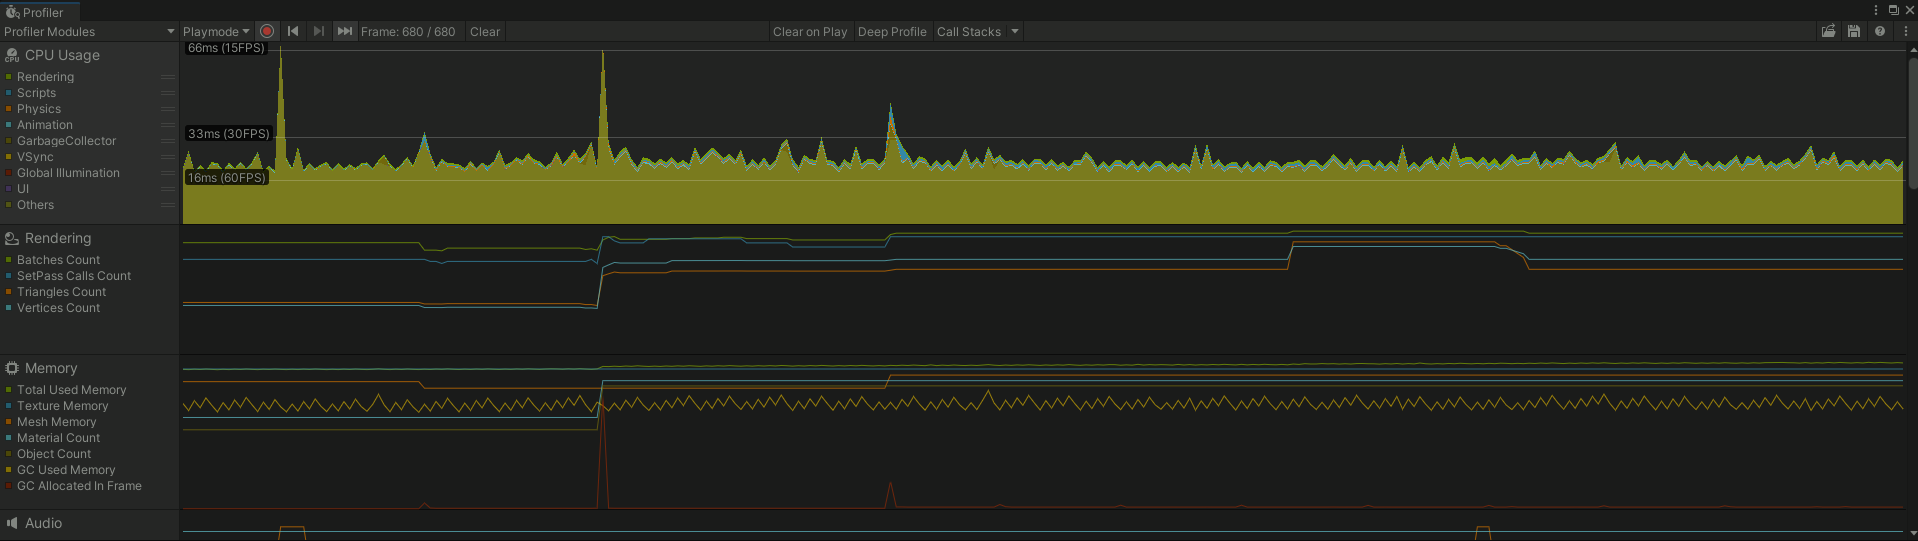
\includegraphics[width=1\linewidth]{"Immagini/ProfilerFPSBassi.png"}
	\caption{Questo è il profiler della simulazione prima dei cambiamenti}
	\label{fig:ProfilerFPSBassi}
\end{figure}
Con il \emph{profiler} alla mano e la simulazione in \emph{play}, si è riusciti a comprendere in quali fasi avesse questi cali drastici. Come primo problema la telecamera era in una pessima angolazione, in alcune zone della tratta la posizione della telecamera le permetteva di inquadrare l'intera mappa, come è possibile vedere dalla Figura \ref{fig:CameraBrutta}, quindi renderizzando l'intero mondo della simulazione sfruttava molte risorse. Si è quindi ridotto la \emph{distanza di render} della telecamera e si è passati ad un'inquadratura a \emph{volo di uccello} facendo sì che non si veda la strada che viene generata.
\begin{figure}[H]
	\centering
	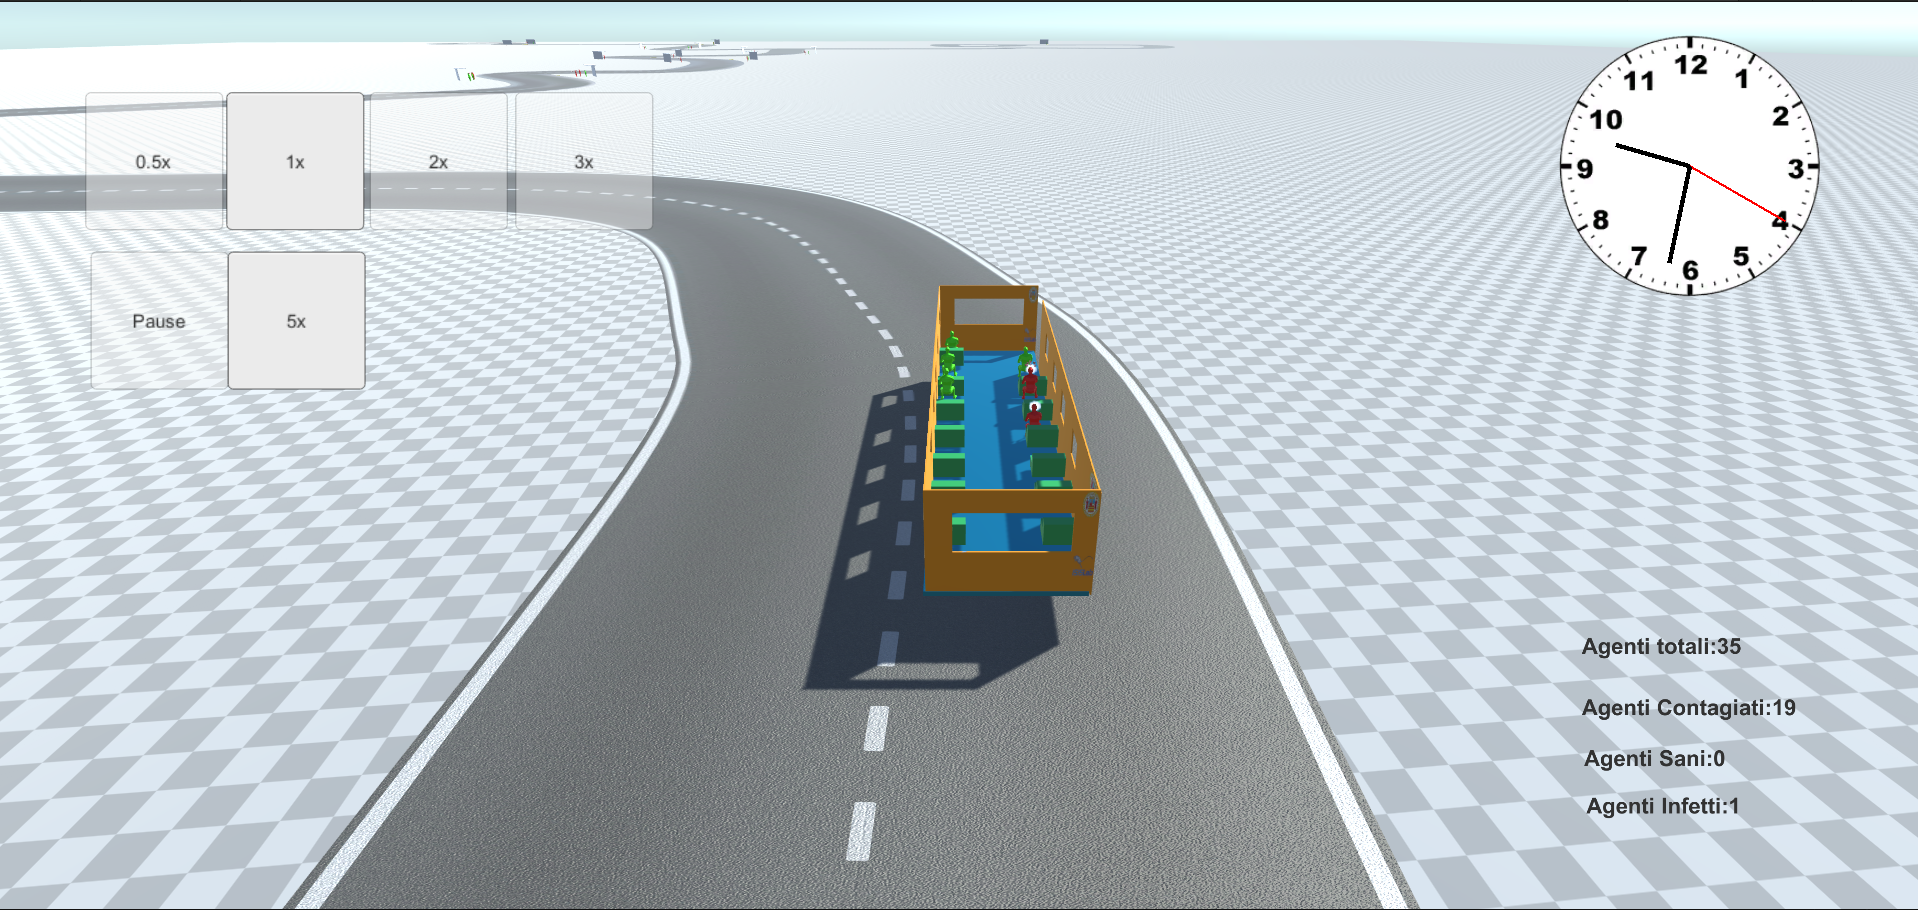
\includegraphics[width=1\linewidth]{"Immagini/CameraBrutta.png"}
	\caption{Questa è un frame nel quale la simulazione perdeva molti frame per secondo}
	\label{fig:CameraBrutta}
\end{figure}
Una volta risolto il problema della telecamera, si è notato che i cali erano, in frequenza minore, ma comunque presenti. Tramite il \textsc{profiler} ci si è accorti che il processo che sfruttava più risorse in certi momenti era il \textsc{particle system}, infatti i frame per secondo si abbassavano quando venivano emesse le particelle. Si è quindi passati a ridurre il numero di particelle emesse, da 10 ad 8, e si è cambiato il modello con il quale venivano generate, non più il modello nella Figura \ref{fig:Covid} ma delle semplici sfere.
\begin{figure}[H]
	\centering
	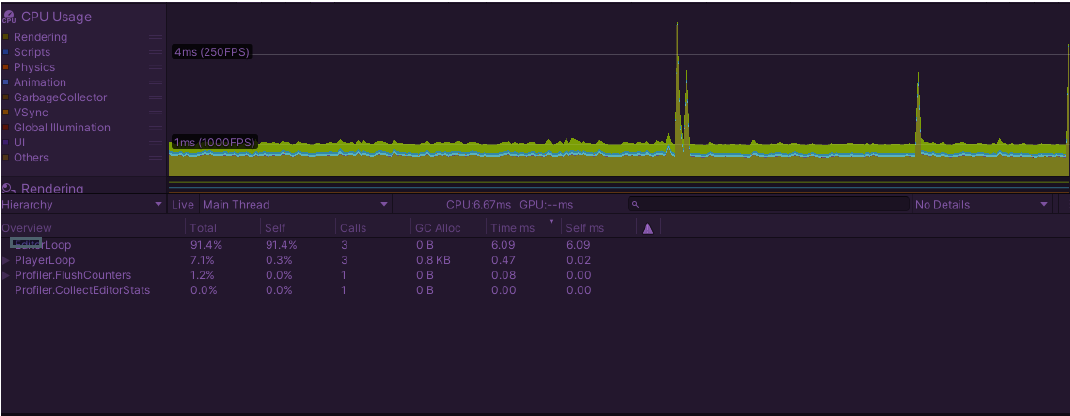
\includegraphics[width=1\linewidth]{"Immagini/ProfilerBuoniFPS.png"}
	\caption{Questo è il profiler della simulazione a 5x}
	\label{fig:ProfilerBuoniFPS}
\end{figure} 
Ora la simulazione ha un'ottima media di frame per secondo, anche a 5x, come è possibile vedere nella Figura \ref{fig:ProfilerBuoniFPS}.

\chapter{Conclusioni}
	In questo capitolo si parlerà dei risultati ottenuti dal progetto, si vedranno dei possibili sviluppi futuri per la simulazione e in conclusione ci saranno considerazioni sull'andamento del lavoro.
	\section{Risultati ottenuti}
	Il principale risultato di questo lavoro è l'aver ottenuto una simulazione, realizzata con l'idea di espandibilità e riutilizzo, in modo tale che possa essere utilizzata come base per ulteriori lavori sulla tematica dei contagi su mezzi di trasporto. Molte componenti della simulazione possono essere trasposti in altri contesti, come ad esempio: la gestione di contagi tramite collider può essere facilmente utilizzata in altri ambiti di simulazioni ad agenti 3D. La possibilità di modificare i parametri della simulazione, tramite una semplice interfaccia, la rende di facile utilizzo per diversi test, i quali risultati sono facilmente utilizzabili per fare delle statistiche, dati i file generati dalla simulazione.
	\section{Sviluppi futuri}
	La simulazione può essere migliorata  inserendo dei dati accurati sui diffusione dei contagi. Realizzare una simulazione a lungo termine per avere dati su diversi giorni ed ottenere una media dei dati dell'andamento dei contagi.
	\section{Considerazioni finali}
	Tramite questo progetto, in collaborazione con il mio collega Ciro Maiorino, abbiamo prodotto una simulazione ad Agenti per quanto riguarda i contagi su mezzi di trasporto partendo da zero, senza alcuna conoscenza delle tecnologie da adoperare. Ora, al termine di questo progetto, sono sicuro nel dire che il presente lavoro potrà essere utilizzato in futuro come punto di riferimento e base per progetti più complessi e ampi.
\bibliographystyle{plain}
\bibliography{bib.bib}
\end{document}